% section 3 Effectiveness
In this chapter, the attemption to proof the effectiveness of our proposed electromagnetic-induced type magnetic cloak is denoted.
To confirm the ability of shielding high fields, three significant parameters have been investigated:
\begin{enumerate}
  \item Time Constant. Since electrical induction is applied in the proposed cloak,
  a long enough time constant of the induced current should be ensured.
  \item Shielding Ability. Since the magnetic cloak works as a magnetic shielding equipment,
  the shielding ability is the key function to be questioned.
  \item Effect of Ferromagnet. To maintain the external surrounding fields the magnetization of ferromagnets is adapted,
  of which the effect should be testified.
\end{enumerate}
Different series of experiments and numerical simulation have been conducted respectively to measured each parameter,
of which the theory, method and results are shown in each section.
In the following sections,
the measurement of the time constant is first denoted in 3.1,
that of the shielding ability is followed in 3.2,
and the effect of ferromagnets is described in 3.3.

\newpage
\subsection{Ability of Shielding Stable High Magnetic Fields}
\subsubsection{Purpose}
Although the zero resistance high temperature superconductor tapes are used in EIMC,
electrical resistance still exists at the connected part.
Due to the resistance, the induced current in the superconductor tapes decreased with time.
The descreasing speed of the current in an RC circuit is known to be related to a parameter called the Time Constant.
If the time constant of a coil is large, longer time is required for the current flowing through to change in magnitude.
It can be considered similar to the law of inertia in motion,
in which an object with a large momentum tends to maitain its speed and direction.

When EIMC are used to shield stable fields,
a large time constant should be ensured to allow the induced current and the shielded state stay for long.
The purpose of this section is to confirm this property being large enough from a series of experiments.

\subsubsection{Theory}
To simulate a magnetic cloak working as a magnetic field shielding equipment,
we have conducted an experiment of which the schmetic design is shown in Fig. \ref{fig:experiment}.

To simulate a stable magnetic field, a trapezoid current is imposed on the outer coil,
as shown in Fig. \ref{fig:imposedCurrentExample}.
Additionally, Fig. \ref{fig:DCTimeSeriesExample} shows an example of the measured magnetic field $B_z$ at certain point inside the inner coil.
In which, following the Faraday's law
altering the external field yields current induction on the opposite direction,
which cancels out the imposed field.
\begin{figure}[H]
  \includegraphics[width=17cm, bb=9 9 900 550]{./section3Effectiveness/imposedCurrentExample.png}
  \caption{A example of the imposed trapezoid current.}
  \label{fig:imposedCurrentExample}
\end{figure}
\begin{figure}[H]
  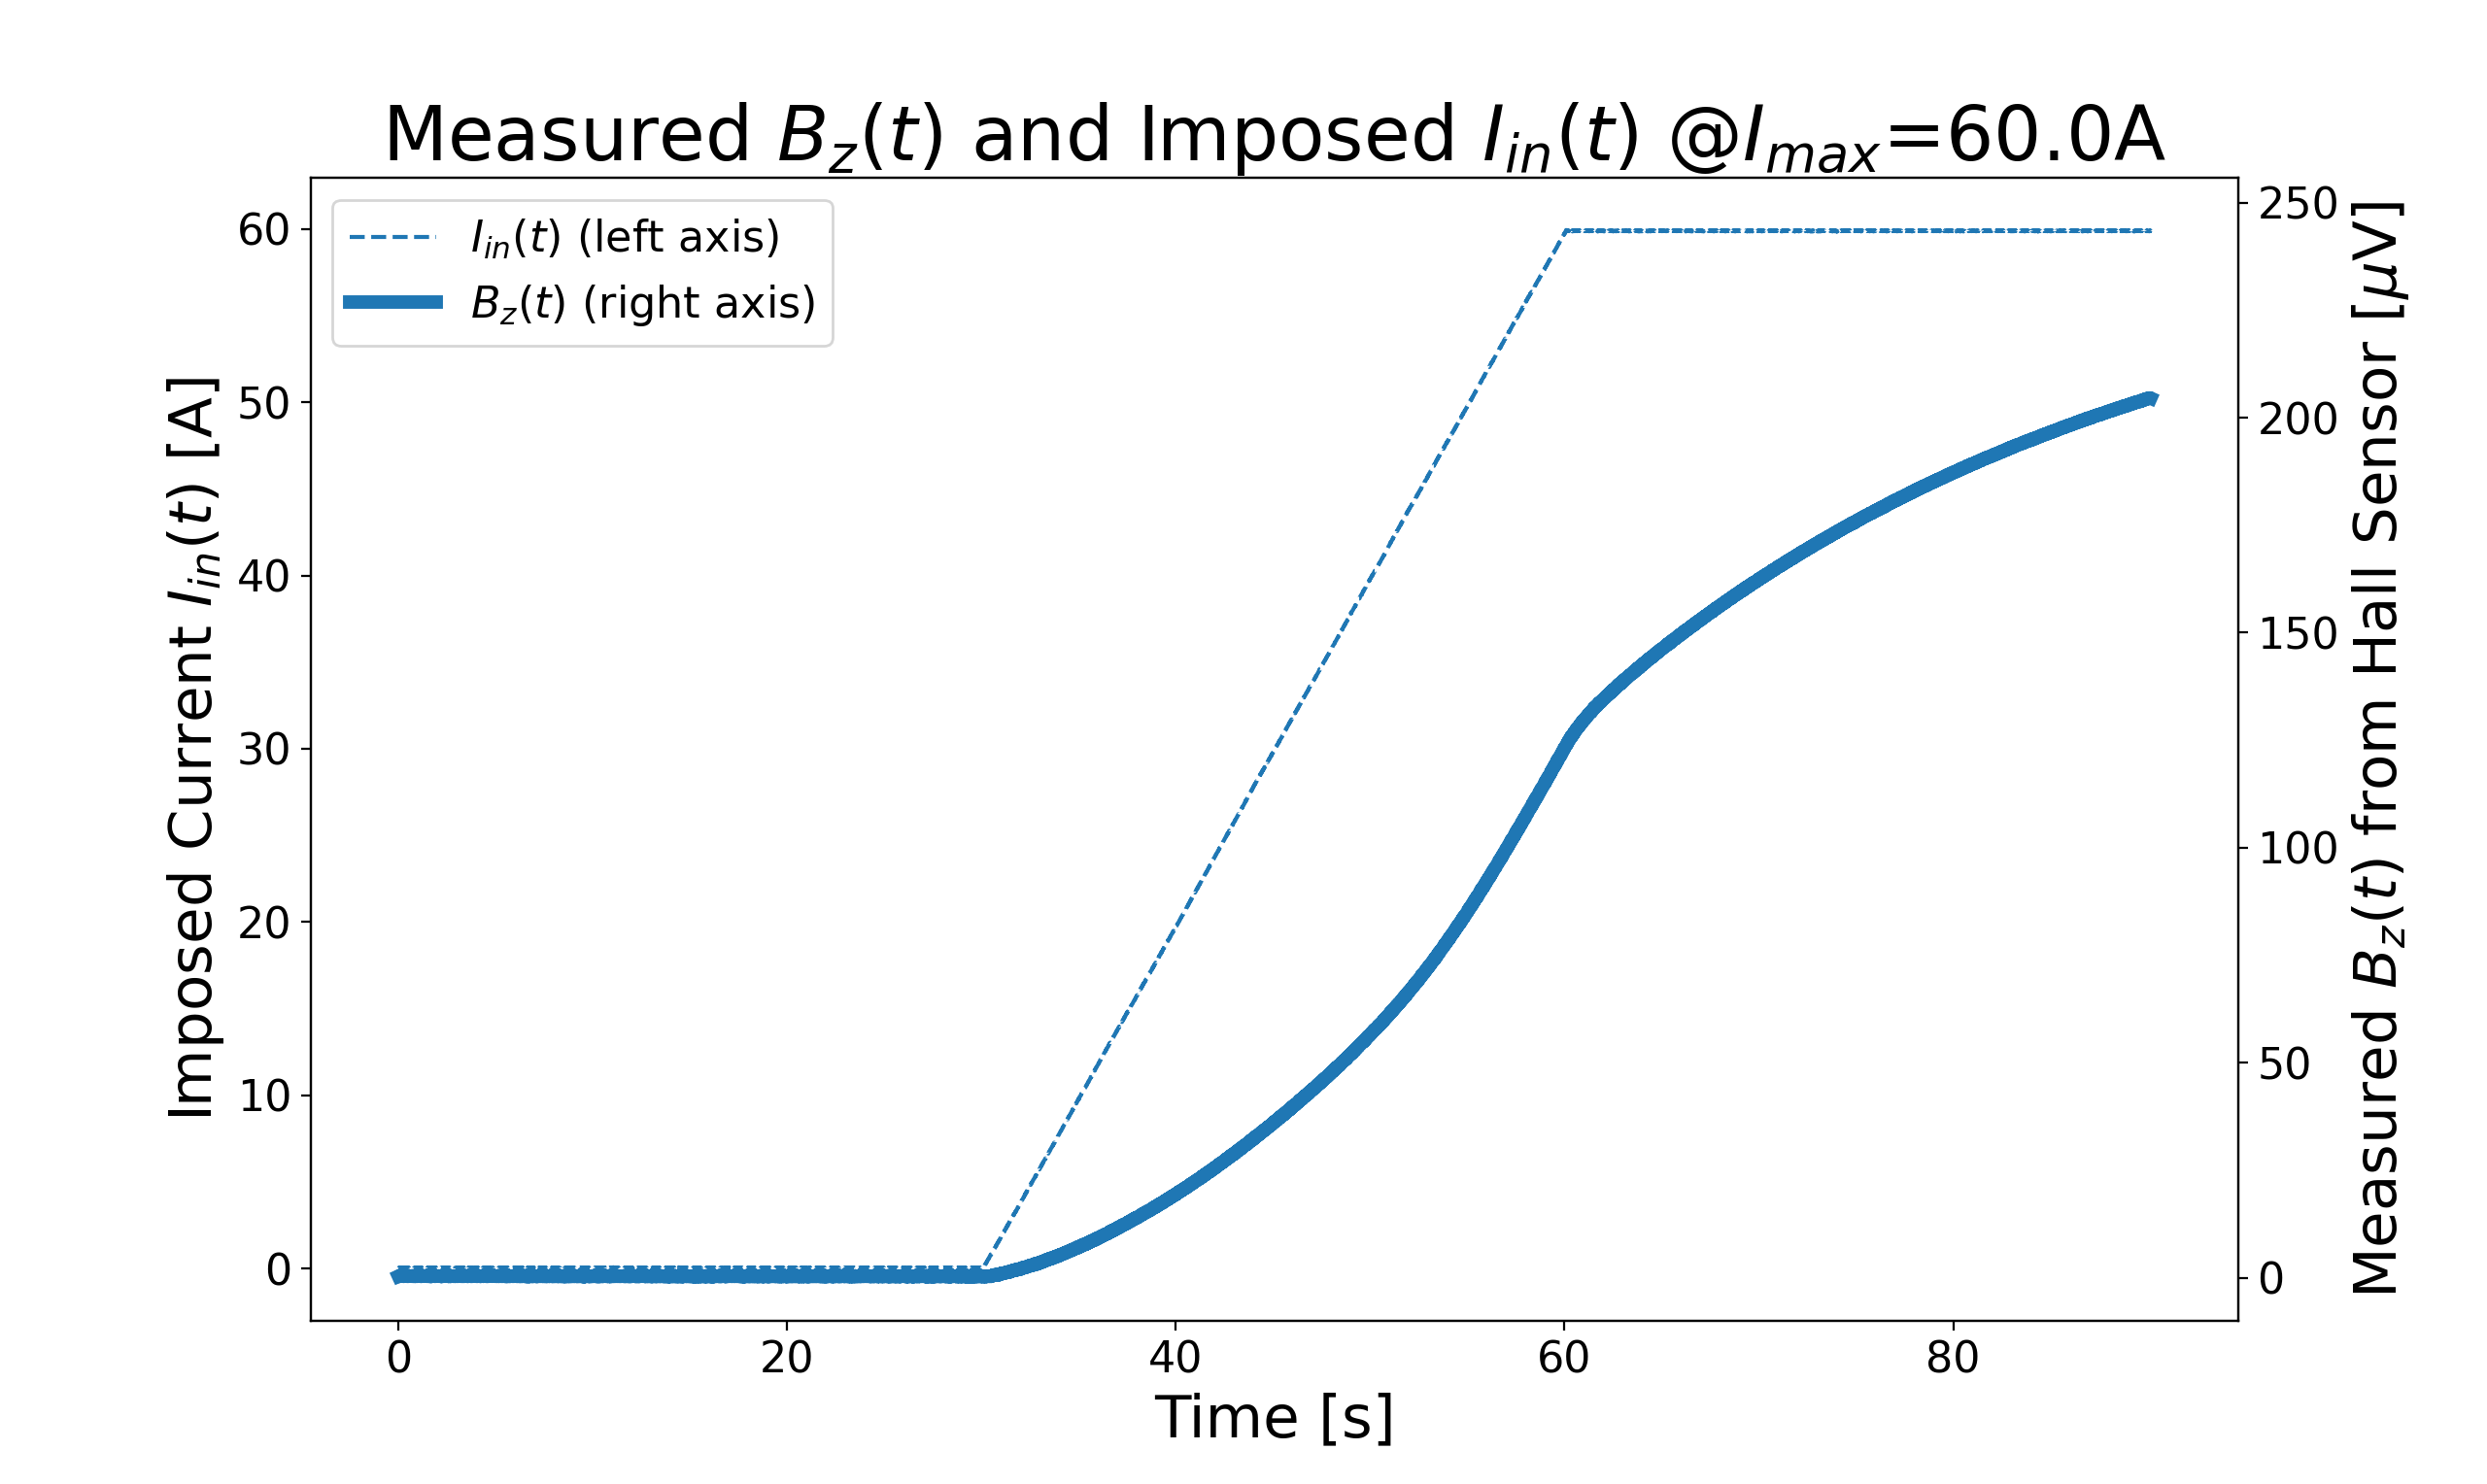
\includegraphics[width=17cm, bb=9 9 900 490]{./section3Effectiveness/DCTimeSeriesExample.png}
  \caption{A example of the magnetic field time variation around the exitation.}
  \label{fig:DCTimeSeriesExample}
\end{figure}

To describe the phenomenen further, a circuit model shown in Fig. \ref{fig:circuit} is taken into advantage.
\begin{figure}[H]
  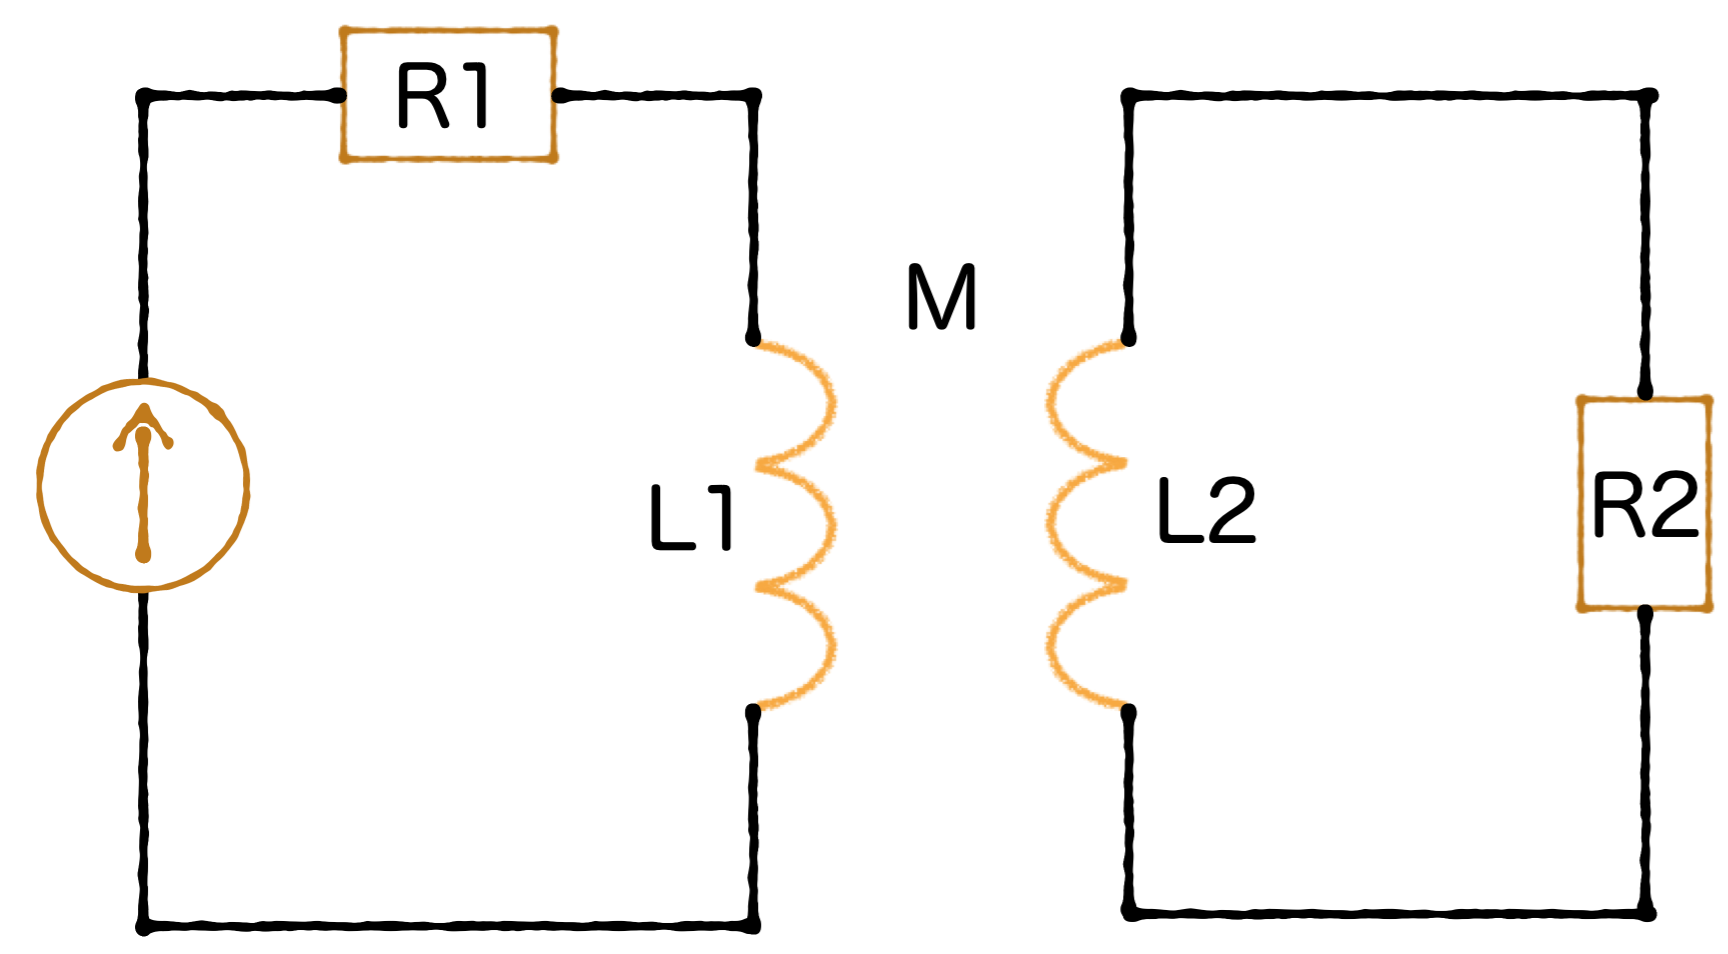
\includegraphics[width=18.5cm, bb=9 9 900 550]{./section3Effectiveness/MLGraph.png}
  \caption{The electrical circuit representing out shielding model.}
  \label{fig:circuit}
\end{figure}
In \ref{fig:circuit}, $R_1$ and $L_1$ stand for the resistance and inductance of the outer coil, and
$R_2$ and $L_2$ stand for the resistance and inductance of inner coil.
When primary current $i_1(t)$ is imposed on the outer coil,
secondary current $i_2(t)$ would be induced on the inner coil through the mutual inductance $M$ between them.
The whole differential equation can be derived as below following the Faraday's law.
\begin{equation}
  L_2\frac{di_2(t)}{dt} + R_2i_2(t) = M\frac{di_1(t)}{dt}
\end{equation}
In our experiment, due to the imposed current being trapezoid,
$M\frac{di_1(t)}{dt}$ is either $0$ or some constant.
Introducing $M\frac{di_1(t)}{dt} = v \in \mathrm{constant}$ into the above equation yields a first order inhomogeneous ordinary differential euqation.
It can be solved by conventional seperation of variables, of which the result (with the initial value considered) is shown below.
\begin{eqnarray}
  i_2(t) = (i_{2_0} &-& \frac{v_2}{R_2})\cdot \exp(-\frac{R_2}{L_2}t) + \frac{v_2}{R_2} \\
  | i_{2_0} &=& i_2(0)\nonumber
\end{eqnarray}
where $i_{2_0}$ is the initial current flowing through the inner coil.

To obtain the induced current $i_2(t)$ in every stage of the trapezoid,
we have modeled the imposed current $i_1(t)$ in all the 5 stages respectively.
The derived results are shown in the equations below.
\begin{eqnarray}
  \mathrm{region1}(t&\in&[0, t_l-\Delta t]): v_2 = 0, i_{2_0} = 0\nonumber\\
  i_2(t) &=& 0\\
  \nonumber\\
  \mathrm{region2}(t&\in&[t_l-\Delta t, t_l]): v_2 = slope_l, i_{2_0} = 0\nonumber\\
  i_2(t) &=& \frac{slope_l}{R_2}\times\left( 1 - \exp(-\frac{R_2}{L_2}(t-(t_l-\Delta t))) \right)\\
  \nonumber\\
  \mathrm{region3}(t&\in&[t_l, t_h]): v_2 = 0, i_{2_0} = i_2(t_l)\nonumber\\
  i_2(t) &=& i_2(t_l)\exp(-\frac{R_2}{L_2}(t-t_l))\\
  \nonumber\\
  \mathrm{region4}(t&\in&[t_h, t_h+\Delta t]): v_2 = slope_h, i_{2_0} = i_2(t_h)\nonumber\\
  i_2(t) &=& \left(i_2(t_h) - \frac{slope_h}{R_2}\right)\exp(-\frac{R_2}{L_2}(t-t_h)) + \frac{slope_h}{R_2}\\
  \nonumber\\
  \mathrm{region5}(t&\in&[t_h+\Delta t, \infty)): v_2 = 0, i_{2_0} = i_2(t_h+\Delta t)\nonumber\\
  i_2(t) &=& i_2(t_h+\Delta t)\exp(-\frac{R_2}{L_2}(t-(t_h+\Delta t)))
\end{eqnarray}
where $t_l$ stands for the end of the exitation, $t_h$ stands for the start of release of imposed current,
$\Delta t$ stands for the exitation time, $I_1$ stands for the peak imposed current,
and $slope_l = -slope_h = M\frac{I_1}{\Delta t}$ holds a meaning of the steepness of the exitation.

By applying Bio-Savart's law to the currents given above, we can derived the expected magnetic fields in all stages.
\begin{eqnarray}
  B(t) &=& C_1\cdot i_1(t) - C_2\cdot i_2(t)\\
  &|& C_1 = \sum_{i=1}^{N1} \frac{\mu_0r_1^2}{2\left(r_1^2 + d_i^2\right)^{\frac{3}{2}}} \in \mathrm{constant}\nonumber\\
  &|& C_2 = \sum_{i=1}^{N2} \frac{\mu_0r_2^2}{2\left(r_2^2 + d_i^2\right)^{\frac{3}{2}}} \in \mathrm{constant}\nonumber
\end{eqnarray}
The total magnetic field $B(t)$ is derived as the summation of the field produced by the inner and outer coil,
which is represented by $C_1i_1(t)$ and $C_2i_2(t)$ respectively.
The coefficients $C_1, C_2 \in \mathrm{constant}$ are parameters related to the shape of the coil,
and can be derived from Bio-Savert's law directly with simple calculation.

Substituting $i_1(t)$ and $i_2(t)$ given by equations (7)-(11) into equation (12) yields the expected field in each stage.
\begin{eqnarray}
  \mathrm{region 1}(t&\in&[0, t_l-\Delta t]):i_1(t) = 0, i_2(t) = 0\nonumber\\
  B(t) &=& 0\\
  \nonumber\\
  \mathrm{region 2}(t&\in&[t_l-\Delta t, t_l]):\nonumber\\
  &|& i_1(t) = \frac{I_1}{\Delta t}(t-t_l) + I_1\nonumber\\
  &|& i_2(t) = \frac{M}{R_2}\cdot\frac{I_1}{\Delta t}\left( 1 - \mathrm{e}^{-\frac{R_2}{L_2}(t-(t_l-\Delta t))}\right)\nonumber\\
  B(t) &=& C_1\cdot\left(\frac{I_1}{\Delta t}(t-t_l) + I_1\right) - C_2\cdot\left( \frac{M}{R_2}\frac{I_1}{\Delta t}\left( 1 - \mathrm{e}^{-\frac{R_2}{L_2}(t-(t_l-\Delta t))}\right) \right)\\
  \nonumber\\
  \mathrm{region 3}(t&\in&[t_l, t_h]):\nonumber\\
  &|& i_1(t) = I1\nonumber\\
  &|& i_2(t) = i_2(t_l)\cdot\mathrm{e}^{-\frac{R_2}{L_2}(t-t_l)}\nonumber\\
  &|& i_2(t_l) = \frac{MI_1}{R_2\Delta t}\left( 1-\mathrm{e}^{-\frac{R_2}{L_2}\Delta t} \right)\in \mathrm{constant}\nonumber\\
  B(t) &=& C_1\cdot I_1 - C_2\cdot\frac{MI_1}{R_2\Delta t}\left( 1-\mathrm{e}^{-\frac{R_2}{L_2}\Delta t} \right)\mathrm{e}^{-\frac{R_2}{L_2}(t-t_l)}
\end{eqnarray}
\begin{eqnarray}
  \mathrm{region 4}(t&\in&[t_h, t_h+\Delta t]):\nonumber\\
  &|& i_1(t) = I_1\left( 1-\frac{t-t_h}{\Delta t} \right)\nonumber\\
  &|& i_2(t) = \left( i_2(t_h)+\frac{MI_1}{R_2\Delta t}\right)\mathrm{e}^{-\frac{R_2}{L_2}(t-t_h)} - \frac{MI_1}{R_2\Delta t} \nonumber\\
  &|& i_2(t_h) = \frac{MI_1}{R_2\Delta t}\left( 1-\mathrm{e}^{-\frac{R_2}{L_2}\Delta t} \right)\mathrm{e}^{-\frac{R_2}{L_2}(t_h-t_l)}\in\mathrm{constant}\nonumber\\
  B(t) &=& C_1\cdot I_1\left( 1-\frac{t-t_h}{\Delta t} \right) - C_2\cdot\left( \left(i_2(t_h)+\frac{MI_1}{R_2\Delta t}\right)\mathrm{e}^{-\frac{R_2}{L_2}(t-t_h)} - \frac{MI_1}{R_2\Delta t} \right)\\
  \nonumber\\
  \mathrm{region 5}(t&\in&[t_h+\Delta t, \infty)):\nonumber\\
  &|& i_1(t) = 0\nonumber\\
  &|& i_2(t) = i_2(t_h+\Delta t)\mathrm{e}^{-\frac{R_2}{L_2}(t-(t_h+\Delta t))}\nonumber\\
  &|& i_2(t_h+\Delta t) = \frac{MI_1}{R\Delta t}\nonumber\\
  &\cdot&\left(\left( 1 -\mathrm{e}^{-\frac{R_2}{L_2}\Delta t} \right)\mathrm{e}^{-\frac{R_2}{L_2}(t_h-t_l)} + \mathrm{e}^{-\frac{R_2}{L_2}\Delta t} - 1 \right)\nonumber\\
  B(t) &=& -C_2\cdot i_2(t_h+\Delta t)\mathrm{e}^{-\frac{R_2}{L_2}(t-(t_h+\Delta t))}
\end{eqnarray}
To make theese equations clear, we have introduced three parameters with physical meaning.
\begin{eqnarray}
  \tau &=& \frac{L_2}{R_2} \mathrm{(time constant)}\\
  \alpha &=& C1\cdot I1 \mathrm{(field produced by the outer coil)}\\
  \beta &=& C2\cdot\frac{MI_1}{R_2\Delta t} \mathrm{(field produced by the inner coil)}
\end{eqnarray}
Introducing theese parameters into equation (13)-(17) yields
\begin{eqnarray}
  \mathrm{region1}(t&\in&[0, t_l-\Delta t]):\nonumber\\
  B(t) &=& 0\\
  \nonumber\\
  \mathrm{region2}(t&\in&[t_l-\Delta t, t_l]):\nonumber\\
  B(t) &=& \alpha\left(\frac{t-t_l}{\Delta t} + 1\right) - \beta\left( 1 - \mathrm{e}^{-\frac{R_2}{L_2}(t-(t_l-\Delta t))}\right)\\
  \nonumber\\
  \mathrm{region3}(t&\in&[t_l, t_h]):\nonumber\\
  B(t) &=& \alpha - \beta\left( 1-\mathrm{e}^{-\frac{\Delta t}{\tau}} \right)\mathrm{e}^{-\frac{t-t_l}{\tau}}\\
  \nonumber\\
  \mathrm{region4}(t&\in&[t_h, t_h+\Delta t]):\nonumber\\
  B(t) &=& \alpha\left( 1-\frac{t-t_h}{\Delta t} \right) - \left( \beta\left(1-\mathrm{e}^{-\frac{\Delta t}{\tau}}\right)\mathrm{e}^{-\frac{t_h-t_l}{\tau}} + \beta \right)\mathrm{e}^{-\frac{t-t_h}{\tau}} + \beta\\
  \nonumber\\
  \mathrm{region5}(t&\in&[t_h+\Delta t, \infty)):\nonumber\\
  B(t) &=& -\beta\left( \left(1-\mathrm{e}^{-\frac{\Delta t}{\tau}}\right)\mathrm{e}^{-\frac{t_h-t_l}{\tau}} + \mathrm{e}^{-\frac{\Delta t}{\tau}} -1 \right) \times\mathrm{e}^{-\frac{t-(t_h+\Delta t)}{\tau}}
\end{eqnarray}
Theese equations (21)-(25) describes the expected magnetic field at the central point if imposed by trapezoid current on the outer coil.


\subsubsection{Method}
A series of experiments have been conducted to measured the time constant.
The experimental equipments are shown in Fig. \ref{fig:experimentalEquipments}.
\begin{figure}[H]
  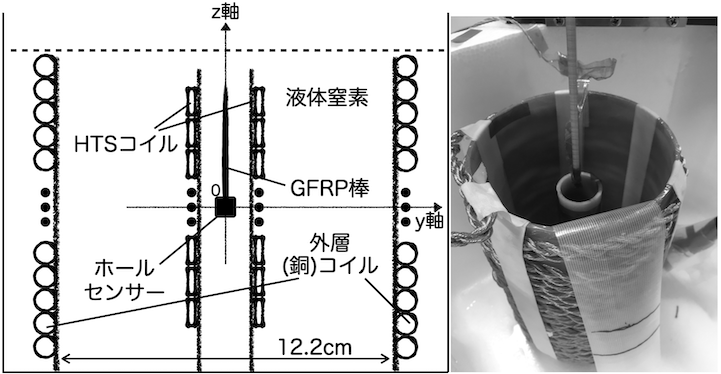
\includegraphics[width=18.5cm, bb=9 9 900 550]{./section3Effectiveness/experimentalEquipments.png}
  \caption{The experimental equipments. (left) The schematic drawing; (right) The photo of which.}
  \label{fig:experimentalEquipments}
\end{figure}
The experiment is conducted in the following procedure on two coils,
one having a small radius and long length, the other owning the opposite.
The specification of the coils is shown in Tab. \ref{tab:expSpecification}.
\begin{enumerate}
  \item Imposed trapezoid current on the outer coil.
  \item Measured the time variation of the central magnetic field.
  \item Fit the measured curve by equation (21)-(25) to find the three paraeters $\tau, \alpha, \beta$.
  \item Repeat on different imposed current.
\end{enumerate}
\begin{table}[H]
  \centering
  \caption{Specification of the experiment.}
  \label{tab:expSpecification}
  \begin{tabular}{cccc}\hline\hline
    Parameter & Inner Coil1 & Inner Coil2 & Outer Coil \\\hline
    Diameter [cm] & 8.8 & 3.0 & 12.2\\\hline
    Length [cm] & 1.2 & 10 & 17.8 \\\hline
    Turns & 2 & 50 & 27 \\\hline
    Critical Current $I_C$ [A] & 500 & 30 & Copper \\\hline
    Width of Superconductor Tape & 12 & 4 & -
  \end{tabular}
\end{table}

\subsubsection{Result and Discussion}
Results of measuring time constants of Coil1 and Coil2 are shown in Fig. \ref{fig:Coil1TimeConstant} and Fig. \ref{fig:Coil2TimeConstant}.
\begin{figure}[H]
  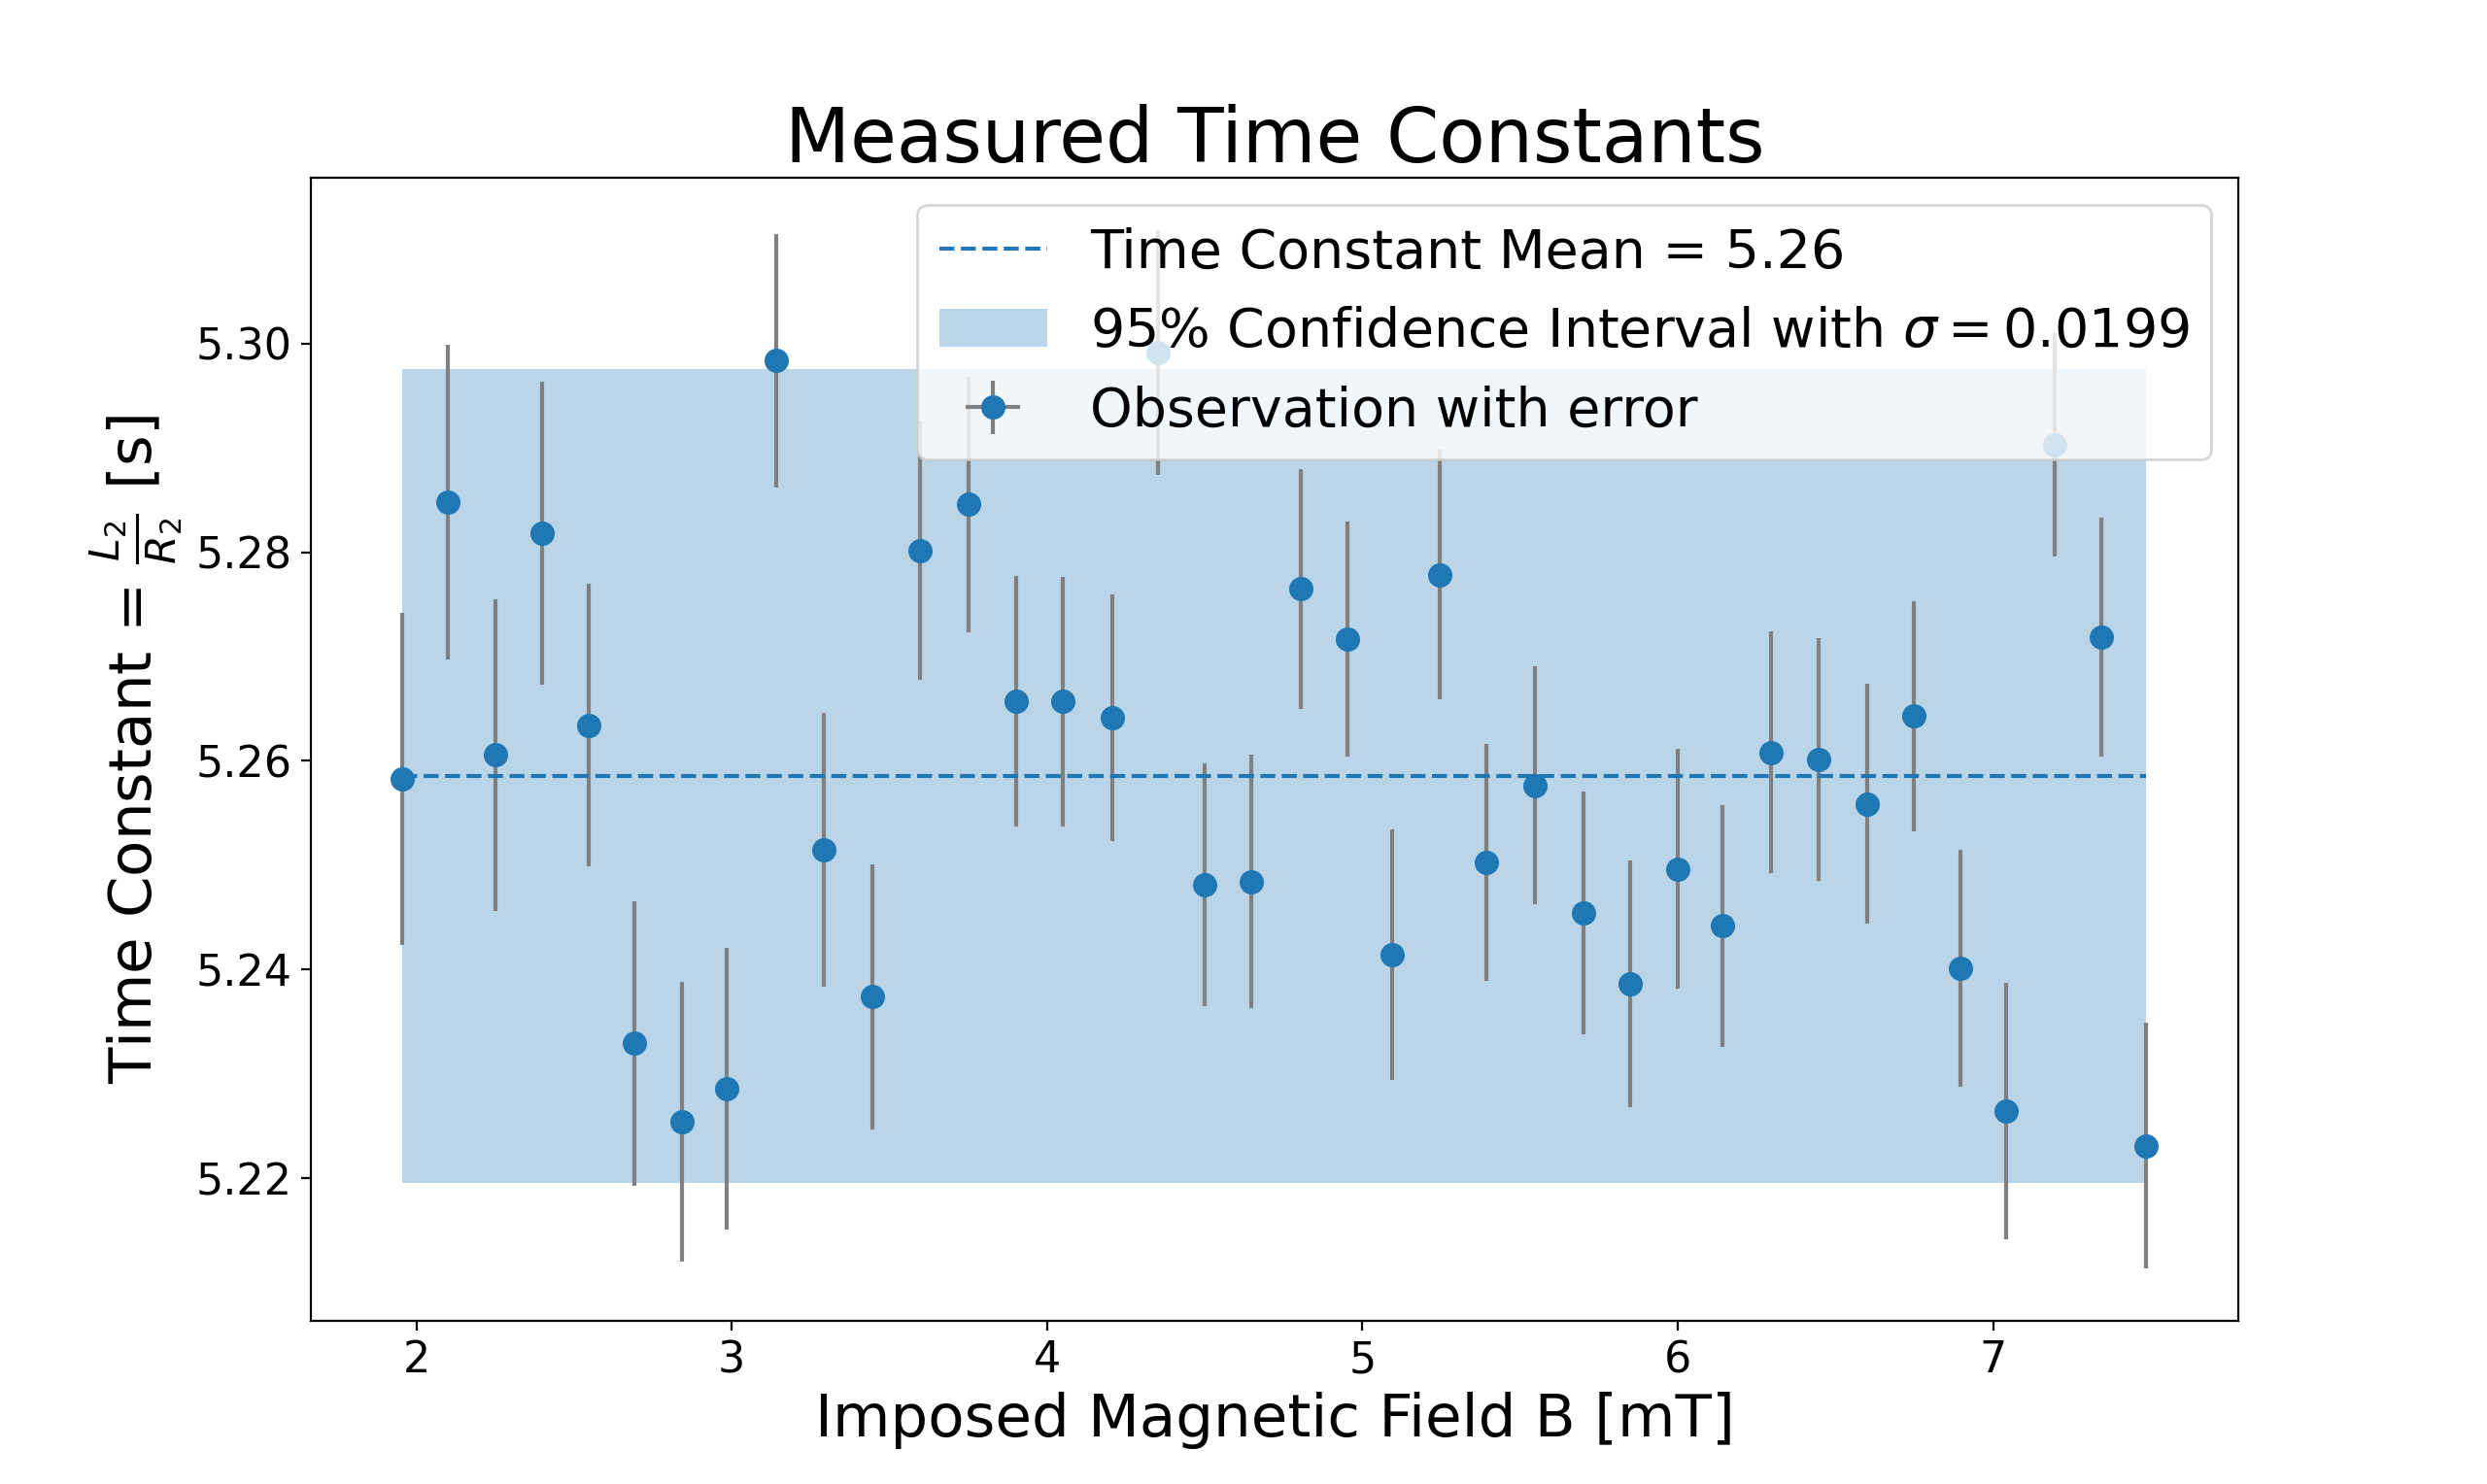
\includegraphics[width=17cm, bb=9 9 900 520]{./section3Effectiveness/Coil1TimeConstant.png}
  \caption{The measured time constant of coil1.}
  \label{fig:Coil1TimeConstant}
\end{figure}
\begin{figure}[H]
  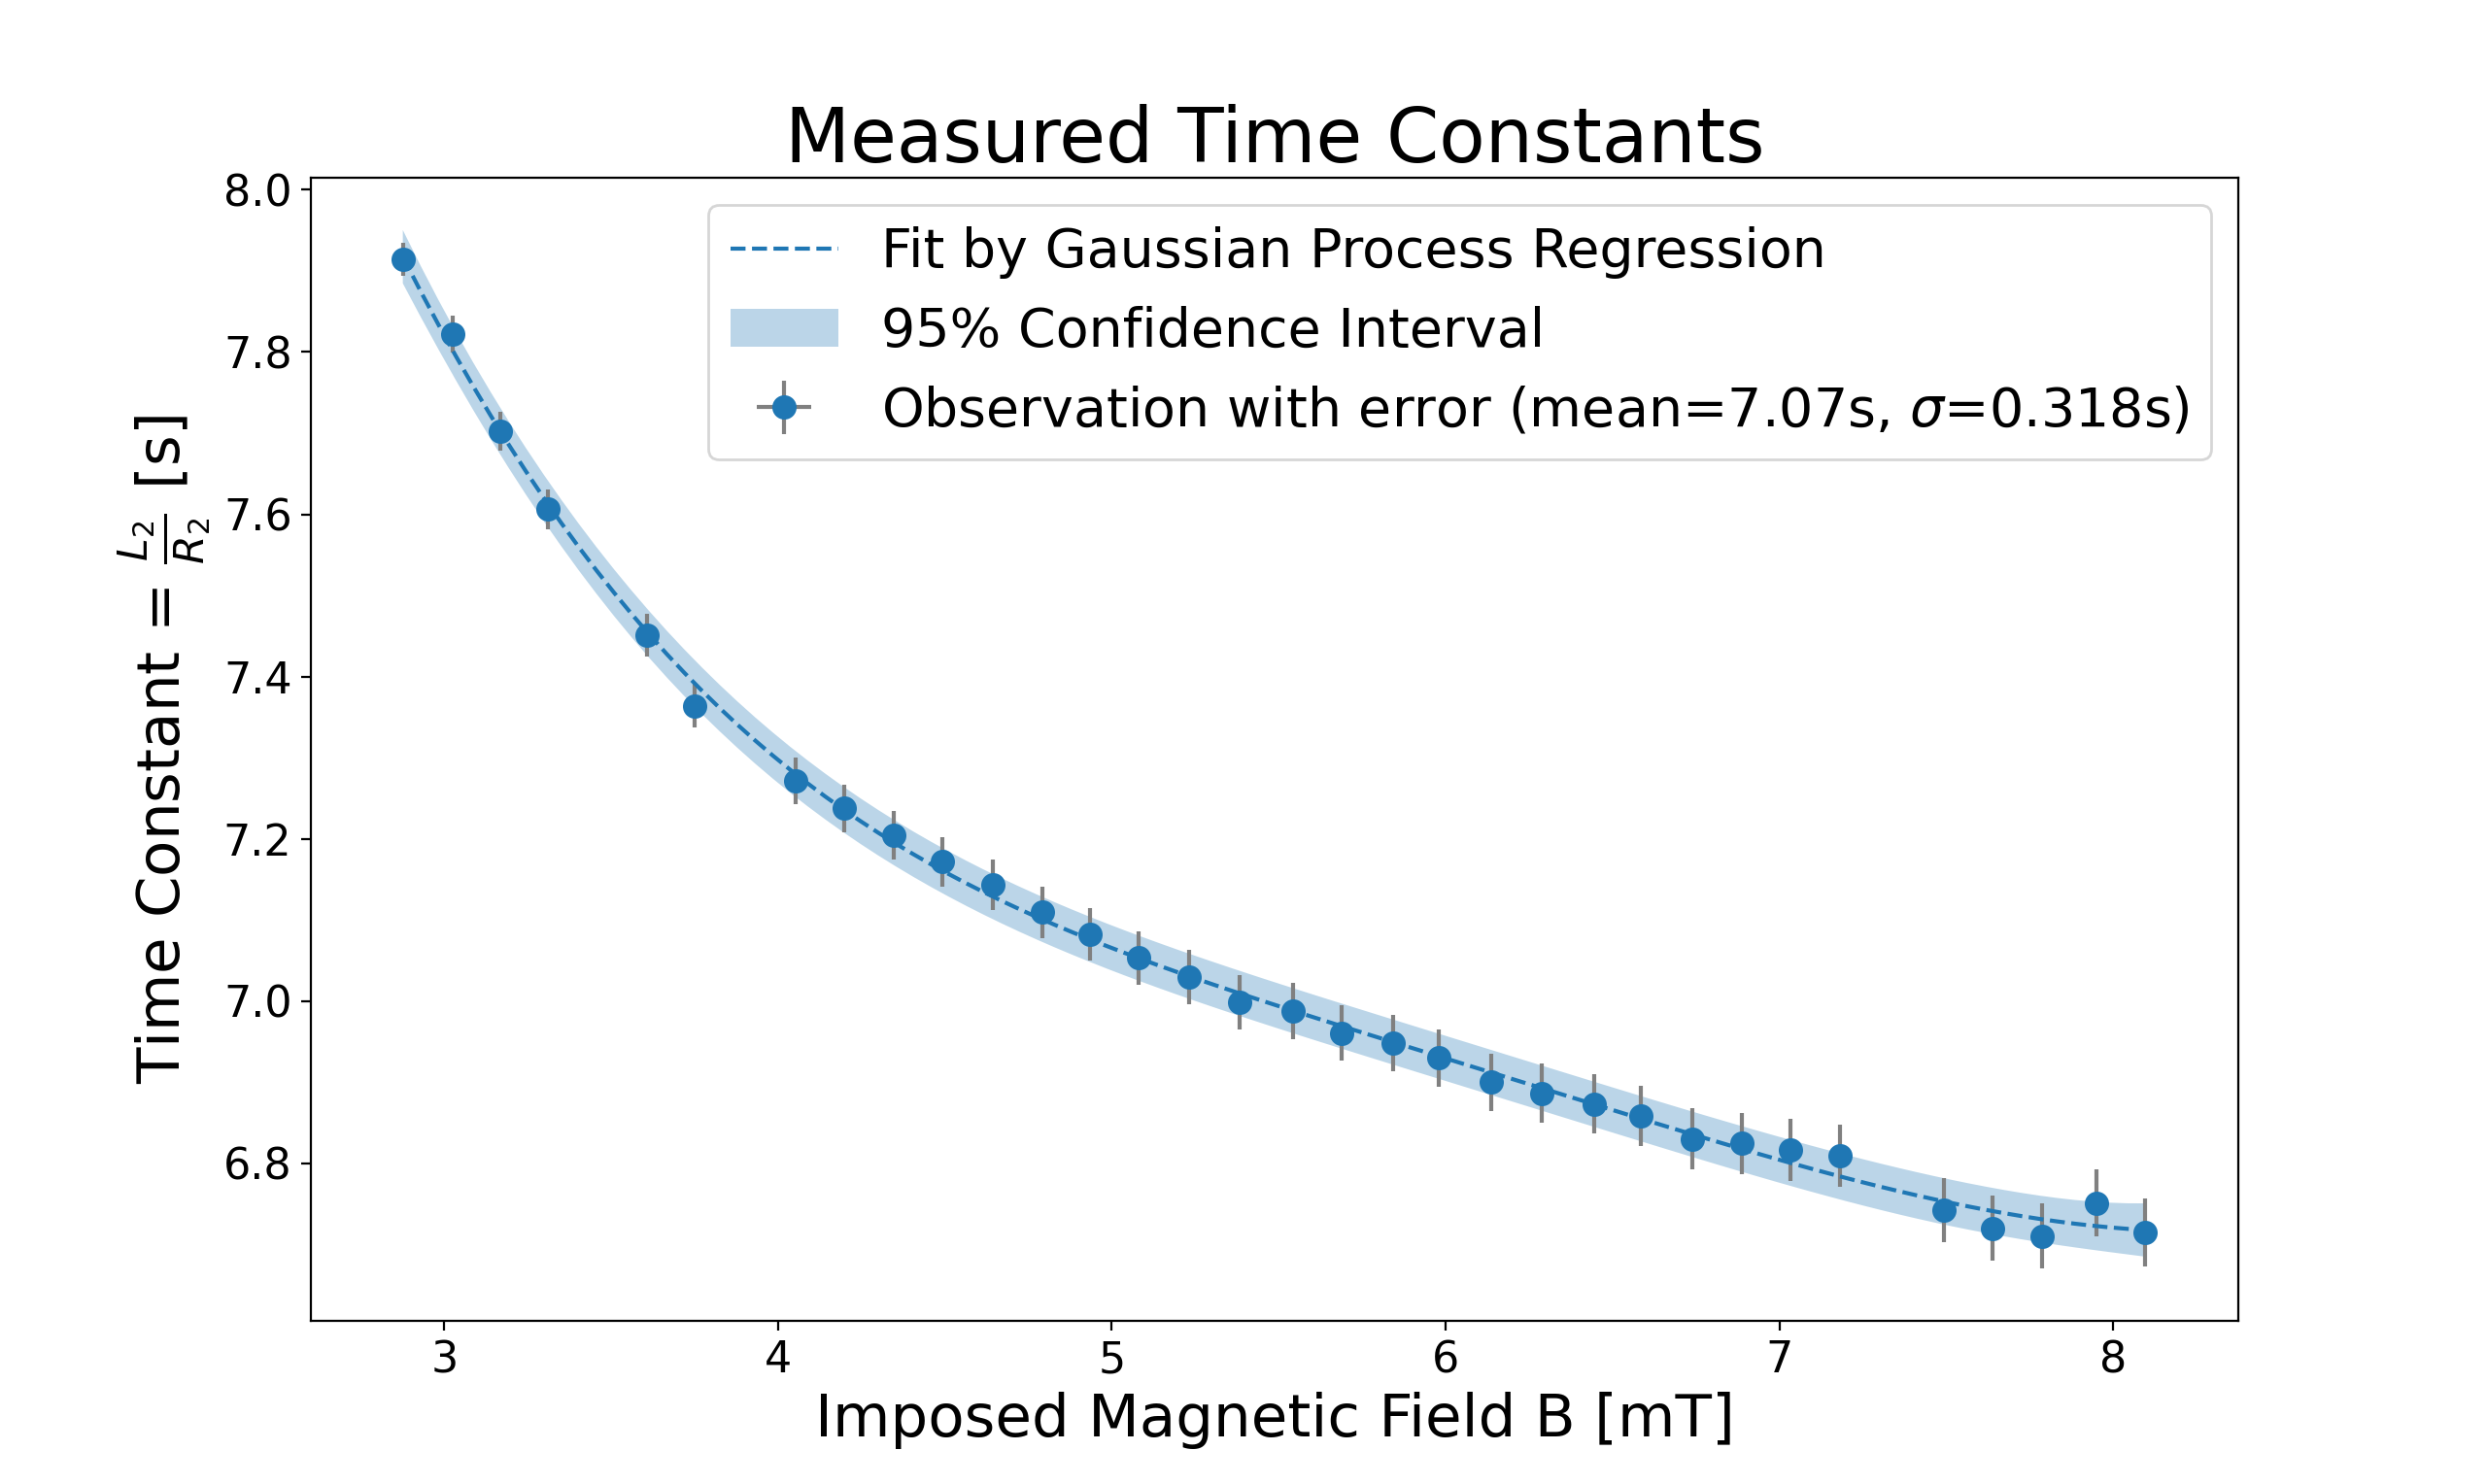
\includegraphics[width=17cm, bb=9 9 900 480]{./section3Effectiveness/Coil2TimeConstant.png}
  \caption{The measured time constant of coil2.}
  \label{fig:Coil2TimeConstant}
\end{figure}
The measured time constant of Coil1 is about $5$ seconds, while that of Coil2 is about $7$ seconds.
In electrical circuits consist of inductance and resistance, the time constant can be written as $\tau = \frac{L}{R}$
Obviously, the difference between them result from the different inductance and resistance of them.
Coil2 has more turns than Coil1, which increases the time constant, but is slightly canceled out by its thinner contact area,
which reduces its time constant.
Besides, the measurement conducted on Coil1 seems to be more stable along different imposed fields,
which in turn gives a more accurate result.
The reason why the time constant of Coil2 shows a magnetic field related property,
which shouldn't happend since both the inductance and the resistance relate only to the shape of coil not the current or any field,
is worth discussed.
One possible hypothesis is due to the non-linearity resistance observed widely on high temperature superconductors.
If we plotted the V-I diagram on superconductor, we would obtain a curve not a straight line,
which indicates the resistance $R = V/I$ is not linear.
Also, When current flow through a superconductor tape increases,
it tends to gather around the surface, which may cause a current related change on inductance.
Either change on the inductance or the resistance will alter the time constant,
this may considered a propper theory.

Besides, another possible reason which rises from the fitting algorithm can be considered.
Since we fit the three parameters from the data simultaneously,
an equaled amount of information on each parameter should be provided properly.
For instance, if a model aimed to recognize either a picture is showing a dog or a cat is trained by 90 dog pictures and 10 cat pictures,
the model tends to give a 90$\%$ guess on dog given any picture,
which is extremely inaccurate.
This is known as the "overfitting" on machine learning field.
In our experiment, we have used the imposed current - measured magnetic field data to find the three parameters,
an equaled amount of information given on them should be guaranteed.

Before we closed this section, the obtained result would be compared with the full scale model to answer the key question:
Is the time constant large enough?
In Fig. \ref{fig:Coil1TimeConstant} and Fig. \ref{fig:Coil1TimeConstant}, we have measured a time constant of a few seconds in both coils.
In our scaled down coils, due to the small inductance and the relatively large electrical resistance,
small time constants of a few seconds are measured.
In a full scale model, for instance a spaceshuttle, the coil becomes enormous and thus owns large inductance and low relatively resistance.
Here we conduct a simple calculation using the specification of the spaceshuttle Columbia,
of which the length is $37.24$ m, the radius is $17.86$ m.
From a conservative perspective, we gave it an 80\% discount.
Using the measured inductance and resistance in the scaled down model,
we are able to derive the full scale time constant as shown below.
\begin{eqnarray}
  \Phi &=& 17.86[\mathrm{m}] \times 80\% = 14.29[\mathrm{m}] \\\nonumber
  \mathrm{length} &=& 37.24[\mathrm{m}] \times 80\% = 29.79[\mathrm{m}] \\\nonumber
  L_{\mathrm{fullScale}} &=& k_N\cdot\frac{\mu N^2\pi r^2}{\mathrm{length}}\cong21.8 [\mathrm{H}] \\\nonumber
  \tau_{\mathrm{real}} &=& \tau_{\mathrm{scaledDown}}\cdot\frac{L_{\mathrm{real}}}{L_\mathrm{scaledDown}} = 5.26[\mathrm{sec}]\cdot\frac{21.8[\mathrm{H}]}{0.4[\mathrm{\mu H}]}\cong 8.7[\mathrm{year}]
\end{eqnarray}
From equation (), a time constant of a few years in a full scale model can be derived,
which indicates that the induced current should retain for a few years making the shielding system feasible.

\subsubsection{Conclusion}
In this section, to give an approximation on the time constant of a full scale model used in space crafts,
we have conducted experiments on 2 scaled down model coil and measured their time constants.
According to the results shown in Fig. \ref{fig:Coil1TimeConstant} and Fig. \ref{fig:Coil1TimeConstant},
the time constants are a few seconds in the scaled down models,
and are calculated to be a few years in a full scale model.
The result infers that the induced current should maintain strengthful for a few years,
showing that the shielding system is capable of working for long enough on every exitation.


\newpage
\subsection{Shielding Ability}
Besides having a large time constant,
performing enough shielding ability is also a critical factor when working as a shielding system.
To testify this property,  a series of experiments have been conducted on mutiple coils.
In this section, we would denote the theory and methods of our experiments as well as the obtain results and the comparison to the full scale model.

\subsubsection{Purpose}
The purpose of this exam is to testify whether the proposed Electromagnetic Induction Type Magnetic Cloak has enough shielding ability.
In theory, shielding rates could reach as high as 99\%, which means shielding 1 T external field to 10 mT is possible.
For convenience, we only take the axis shielding rate into evaluation,
since the measured field in the entire internal space would be no difference beyond 10\%.

\subsubsection{Theory}
The entire circuit is the same as Fig. \ref{fig:experiment} in section 3.1 except for the imposed current being AC instead of DC.
If AC current $i_1(t) = I_1\sin(\omega t)$ is imposed, equation (5) becomes a classic Bernoulli equation,
which can be solved by introducing propper intergrating factor.
The general solution with initial value involved is shown below.
\begin{eqnarray}
  i_2(t) &=& \mathrm{e}^{-h(t)}\left( \int \mathrm{e}^{h(t)}\cdot r(t)dt + C_0 \right)\nonumber\\
  &|& h(t) = \frac{R_2}{L_2}t, r(t) = \frac{M}{L_2}\cdot I_1\omega\cos(\omega t) \nonumber\\
  &=& \frac{\frac{M}{L_2}\omega I_1}{(\frac{R_2}{L_2})^2+\omega^2}\left(\frac{R_2}{L_2}\right)\mathrm{e}^{-\frac{R_2}{L_2}t} \nonumber\\
  &+& \frac{\frac{M}{L_2}\omega I_1}{(\frac{R_2}{L_2})^2+\omega^2}\left(\frac{R_2}{L_2}\cos(\omega t) + \omega\sin(\omega t)\right)
\end{eqnarray}
This equation describes the induced current $i_2(t)$ when imposed by sin wave.
In equation (27), the first term refers to the transient phenomena with time constant $\tau$,
while the second term represents the steady state.
If the frequency is relatively large $\omega \gg \frac{R_2}{L_2}$,
$i_2(t)$ becomes strictly sin wave shown below,
which agrees with the solution from phasor calculation.
\begin{equation}
  i_2(t) = \frac{MI_1}{L_2}\cdot\sin(\omega t) |\omega \gg \frac{R_2}{L_2}
\end{equation}
By equation (28), we are able to derive the central magnetic field $B(t)$ as below.
\begin{eqnarray}
  B(t) &=& C_1\cdot i_1(t) - C_2\cdot i_2(t)\nonumber\\
  &|& C_1 = \sum_{i=1}^{N1} \frac{\mu_0r_1^2}{2\left(r_1^2 + d_i^2\right)^{\frac{3}{2}}} \in \mathrm{constant}\nonumber\\
  &|& C_2 = \sum_{i=1}^{N2} \frac{\mu_0r_2^2}{2\left(r_2^2 + d_i^2\right)^{\frac{3}{2}}} \in \mathrm{constant}\nonumber\\
  &|& i_1(t) = I_1\sin(\omega t)\nonumber\\
  &|& i_2(t) = \frac{MI_1}{L_2}\cdot\sin(\omega t)\nonumber\\
  &=& C_1\cdot I_1\sin(\omega t) - C_2\cdot\frac{MI_1}{L_2}\sin(\omega t)|\omega \gg \frac{R_2}{L_2}
\end{eqnarray}
where the first term represents the field generated by the external coil,
and the second term represents the field generated by the internal coil.
We can further derive the centeral shielding rate to be
\begin{equation}
  \mathrm{Shielding Rate} = \frac{C_2\cdot i_2(t)}{C1\cdot i_1(t)} = \frac{C_2}{C_1}\cdot\frac{M}{L_2}
\end{equation}
Surprisingly, according to equation (30),
the shielding rate only depends on the shape of the external coil ($C_1$),
the shape of the internal coil ($C_2$),
the mutual inductance between them ($M$),
and the inductance of the internal coil ($L_2$).
Note that given a fix shape external coil,
the shielding rate would be defined by $\frac{C_2M}{L_2}$,
and thus we can't tell anything about how the shielding rate would change when the size of internal coil decreases.
It needs to be calculated case by case, which may become annoying on the system desing.
The detail of coefficients $C_1$ and $C_2$ have already been shown in equation (12).
The derivation of $M$ and $L$ would be shown in the following paragraph.


\begin{figure}[H]
  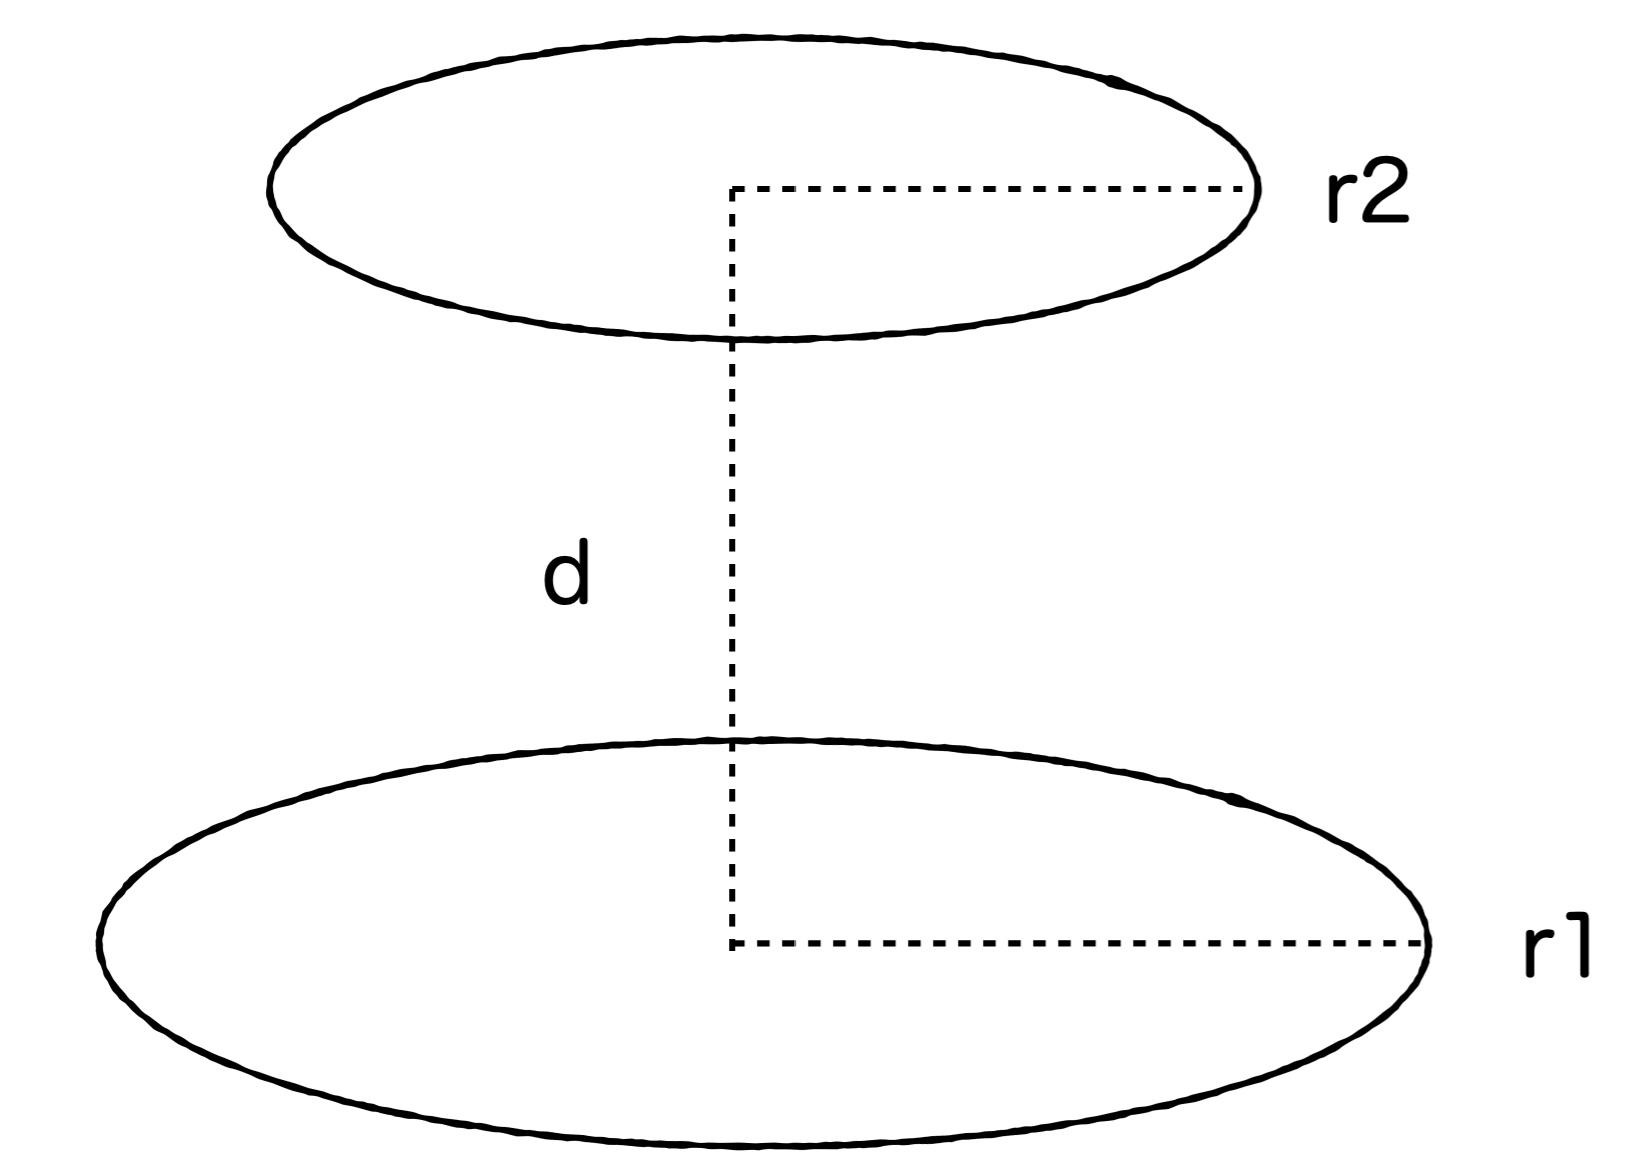
\includegraphics[width=17cm, bb=9 9 900 550]{./section3Effectiveness/2CoilsExample.png}
  \caption{A schematic diagram of mutal inductance derived from 2 loops.}
  \label{fig:M}
\end{figure}
Imagine two conductive loops with radius $r_1$ and $r_2$ respectively, placed parallelly by distance $d$ like Fig. \ref{fig:M}.
The mutual inductance between them could be derived from Neumann's formula.
\begin{eqnarray}
  M(r_1, r_2, d) &=& \frac{\mu_0}{4\pi}\int_0^{2\pi}\int_0^{2\pi} \frac{r_1r_2\cos(\theta-\theta')d\theta d\theta'}{\sqrt{r_1^2 + r_2^2 + d^2 - 2r_1r_2\cos(\theta-\theta')}} \nonumber\\
  &=& \frac{\mu_0}{2}\int_0^{2\pi} \frac{r_1r_2\cos(\phi) d\phi}{\sqrt{r_1^2 + r_2^2 + d^2 - 2r_1r_2\cos(\phi)}}
\end{eqnarray}
This integral couldn't be solved with only elementary functions,
but by introducing elliptic integral it can be rewritten into closed form,
as shown in equation (32).
\begin{eqnarray}
  M(r_1, r_2, d) &=& \mu_0\sqrt{r_1r_2}\left( (\frac{2}{k}-k)K(k) - \frac{2}{k}E(k) \right)\\
  &|& k = \sqrt{\frac{4r_1r_2}{(r_1+r_2)^2 + d^2}}\nonumber\\
  &|& K(k) = \mathrm{The first kind complete elliptic integral with modulus} k\nonumber\\
  &|& E(k) = \mathrm{The second kind complete elliptic integral with modulus} k\nonumber
\end{eqnarray}
Equation (32) denotes the mutual inductance between two loops from the first principles.
For the mutual inductance between two multi-turn coils,
applying equation (32) to all their turn would raise the total mutual inductance.
\begin{eqnarray}
  \sum M &=& \sum_{i=1}^{N_1\cdot N_2}\mu_0\sqrt{r_1r_2}\left( (\frac{2}{k_i}-k_i)K(k_i) - \frac{2}{k_i}E(k_i) \right)\nonumber\\
  &|& k = \sqrt{\frac{4r_1r_2}{(r_1+r_2)^2 + d_i^2}}
\end{eqnarray}
where $d_i$ refers to the central distance betwenn the specific turns,
$N_1$ and $N_2$ refer to the turns of the each coil.
Equation (33) represents the mutual inductance $M$ between $N_1$ turns external coil and $N_2$ turns internal coil.


Next, we derive the inductance $L$ of a finite length $l$ solenoid coil with radius $r$, $N$ turns.
First, the inductance of an infinite solenoid coil $l \to \infty$ is well known as $L = \frac{\mu N^2\pi r^2}{l}$.
When the length is finite, a coefficient $K_N$ ranging from $0\sim1$, named after Nagaoka Hanntaro, should be multiplied.
\begin{eqnarray}
  L&(&r, l) = K_N\cdot\frac{\mu N^2\pi r^2}{l}\\
  &|& K_N = \frac{4}{3\pi\sqrt{1-n^2}}\left( \frac{1-n^2}{n^2}K(n) - \frac{1-2n^2}{n^2}E(n) - n \right)\nonumber\\
  &|& n(r, l) = \frac{1}{\sqrt{(\frac{l}{2r})^2 + 1}}\nonumber\\
  &|& K(n) = \mathrm{TheFirstKindCompleteEllipticIntegralWithModulus} k\nonumber\\
  &|& E(n) = \mathrm{TheSecondKindCompleteEllipticIntegralWithModulus} k\nonumber
\end{eqnarray}
Equation (34) represents the inductance of a $N$ turns, radius $r$, and relatively short length solenoid coil.


Using the equations described in section 3.2.1-3.2.2,
we are able to write the shielding rate from foundamental coil parameters.
\begin{eqnarray}
  \mathrm{Shielding Rate}&(&r_1, l_1, N_1, r_2, l_2, N_2) = \frac{C_2}{C_1}\times\frac{M}{L_2}\\
  &=& \frac{\sum_{i=1}^{N1} \frac{\mu_0r_1^2}{2\left(r_1^2 + d_i^2\right)^{\frac{3}{2}}}}{\sum_{i=1}^{N2} \frac{\mu_0r_2^2}{2\left(r_2^2 + d_i^2\right)^{\frac{3}{2}}}}\nonumber\\
  &\times& \frac{\sum_{i=1}^{N_1\cdot N_2}\mu_0\sqrt{r_1r_2}\left( (\frac{2}{k_i}-k_i)K(k_i) - \frac{2}{k_i}E(k_i) \right)}{K_N\cdot\frac{\mu N^2\pi r^2}{l}}\nonumber
\end{eqnarray}
Given an external coil (radius $r_1$, turns $N_1$, length $l_1$),
and an internal coil (radius $r_2$, turns $N_2$, length $l_2$),
equation (35) explains the central shielding rate when external coil is imposed by $i_1(t) = I_1\sin(\omega t)$.
The shielding rate here is defined as, the field generated by internal coil devided by the field generated by external coil.
As well, equation (35) holds when the frequency $\omega$ is extremely larger than $\tau=\frac{R_2}{L_2}$ is satisfied.

Just as described in 3.2.1, the shielding rate depends on the shapes of both coils and grows nonlinearly,
which is hard to imagine.
To give a schematic picture of it, we have calculated some shielding rates under various internal coils and a fix external coil,
using equation ().
Fig. \ref{fig:simulatedShieldingRates3D1} and \ref{fig:simulatedShieldingRates3D2} shows the same simulated result,
from different angle.
Fig. \ref{fig:overshielding}
\begin{figure}[H]
  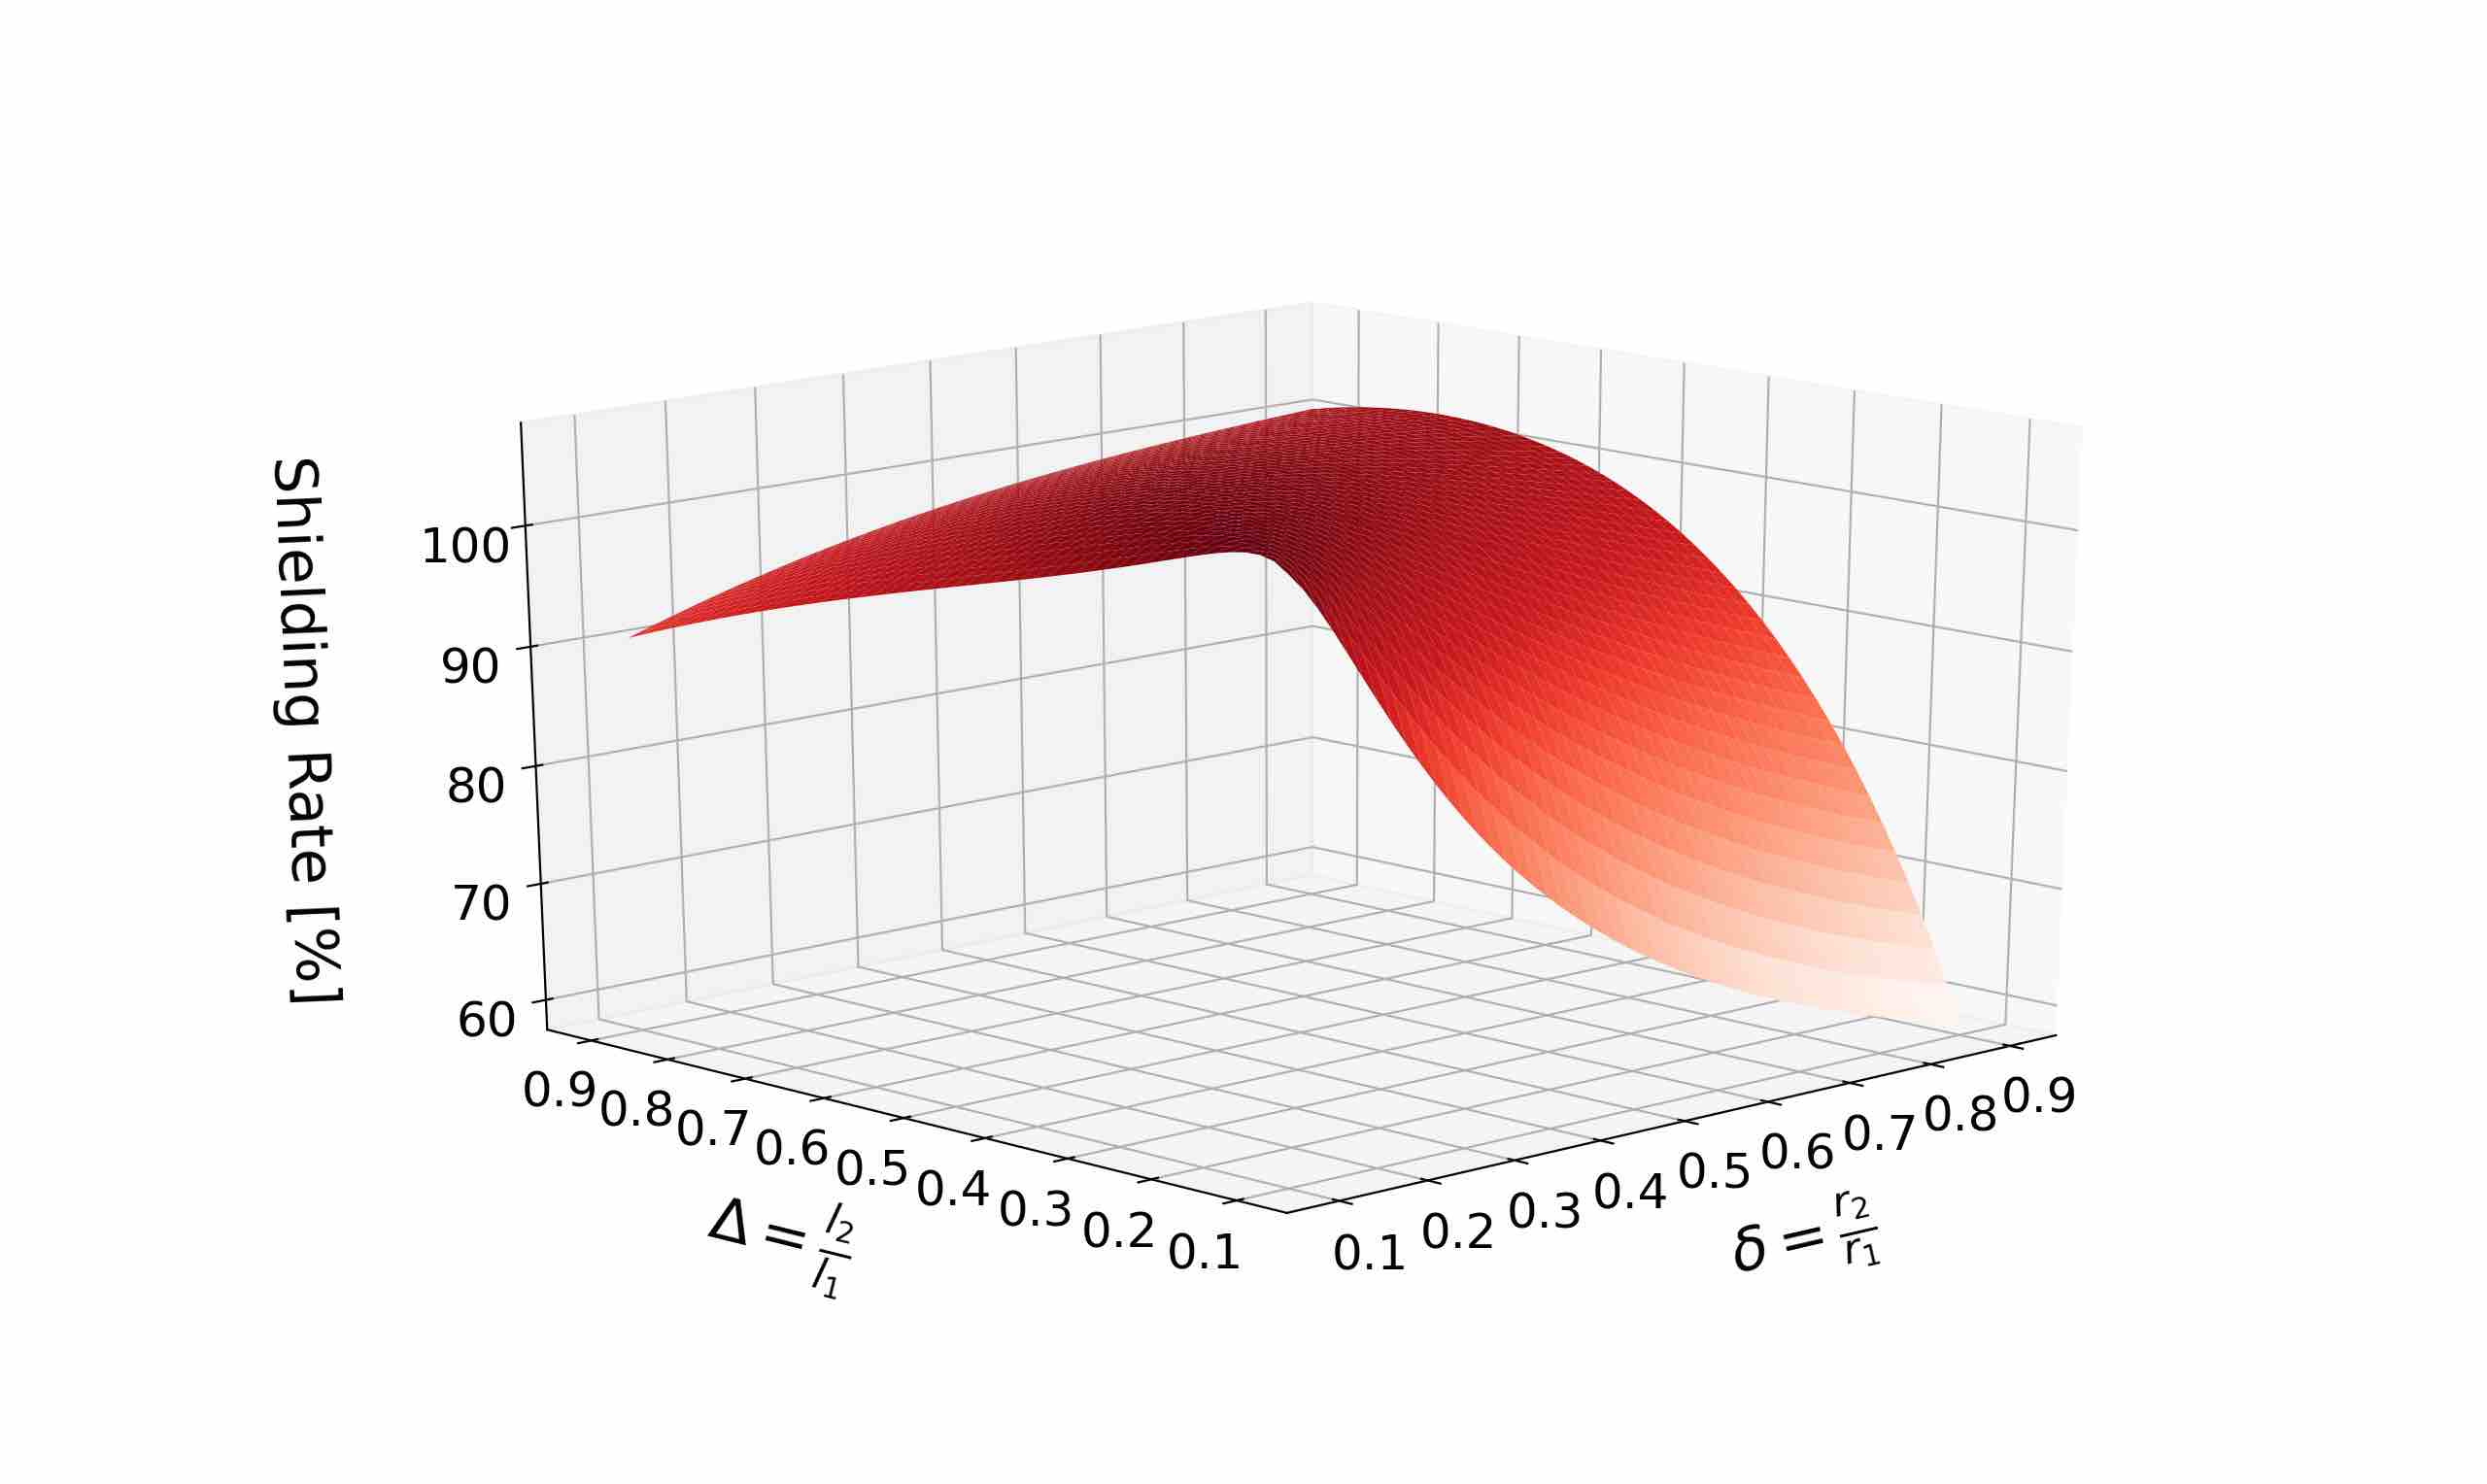
\includegraphics[width=17cm, bb=9 9 900 550]{./section3Effectiveness/simulatedShieldingRates3D1.JPEG}
  \caption{Simulated shielding rates with different $r_2, l_2$.}
  \label{fig:simulatedShieldingRates3D1}
\end{figure}
\begin{figure}[H]
  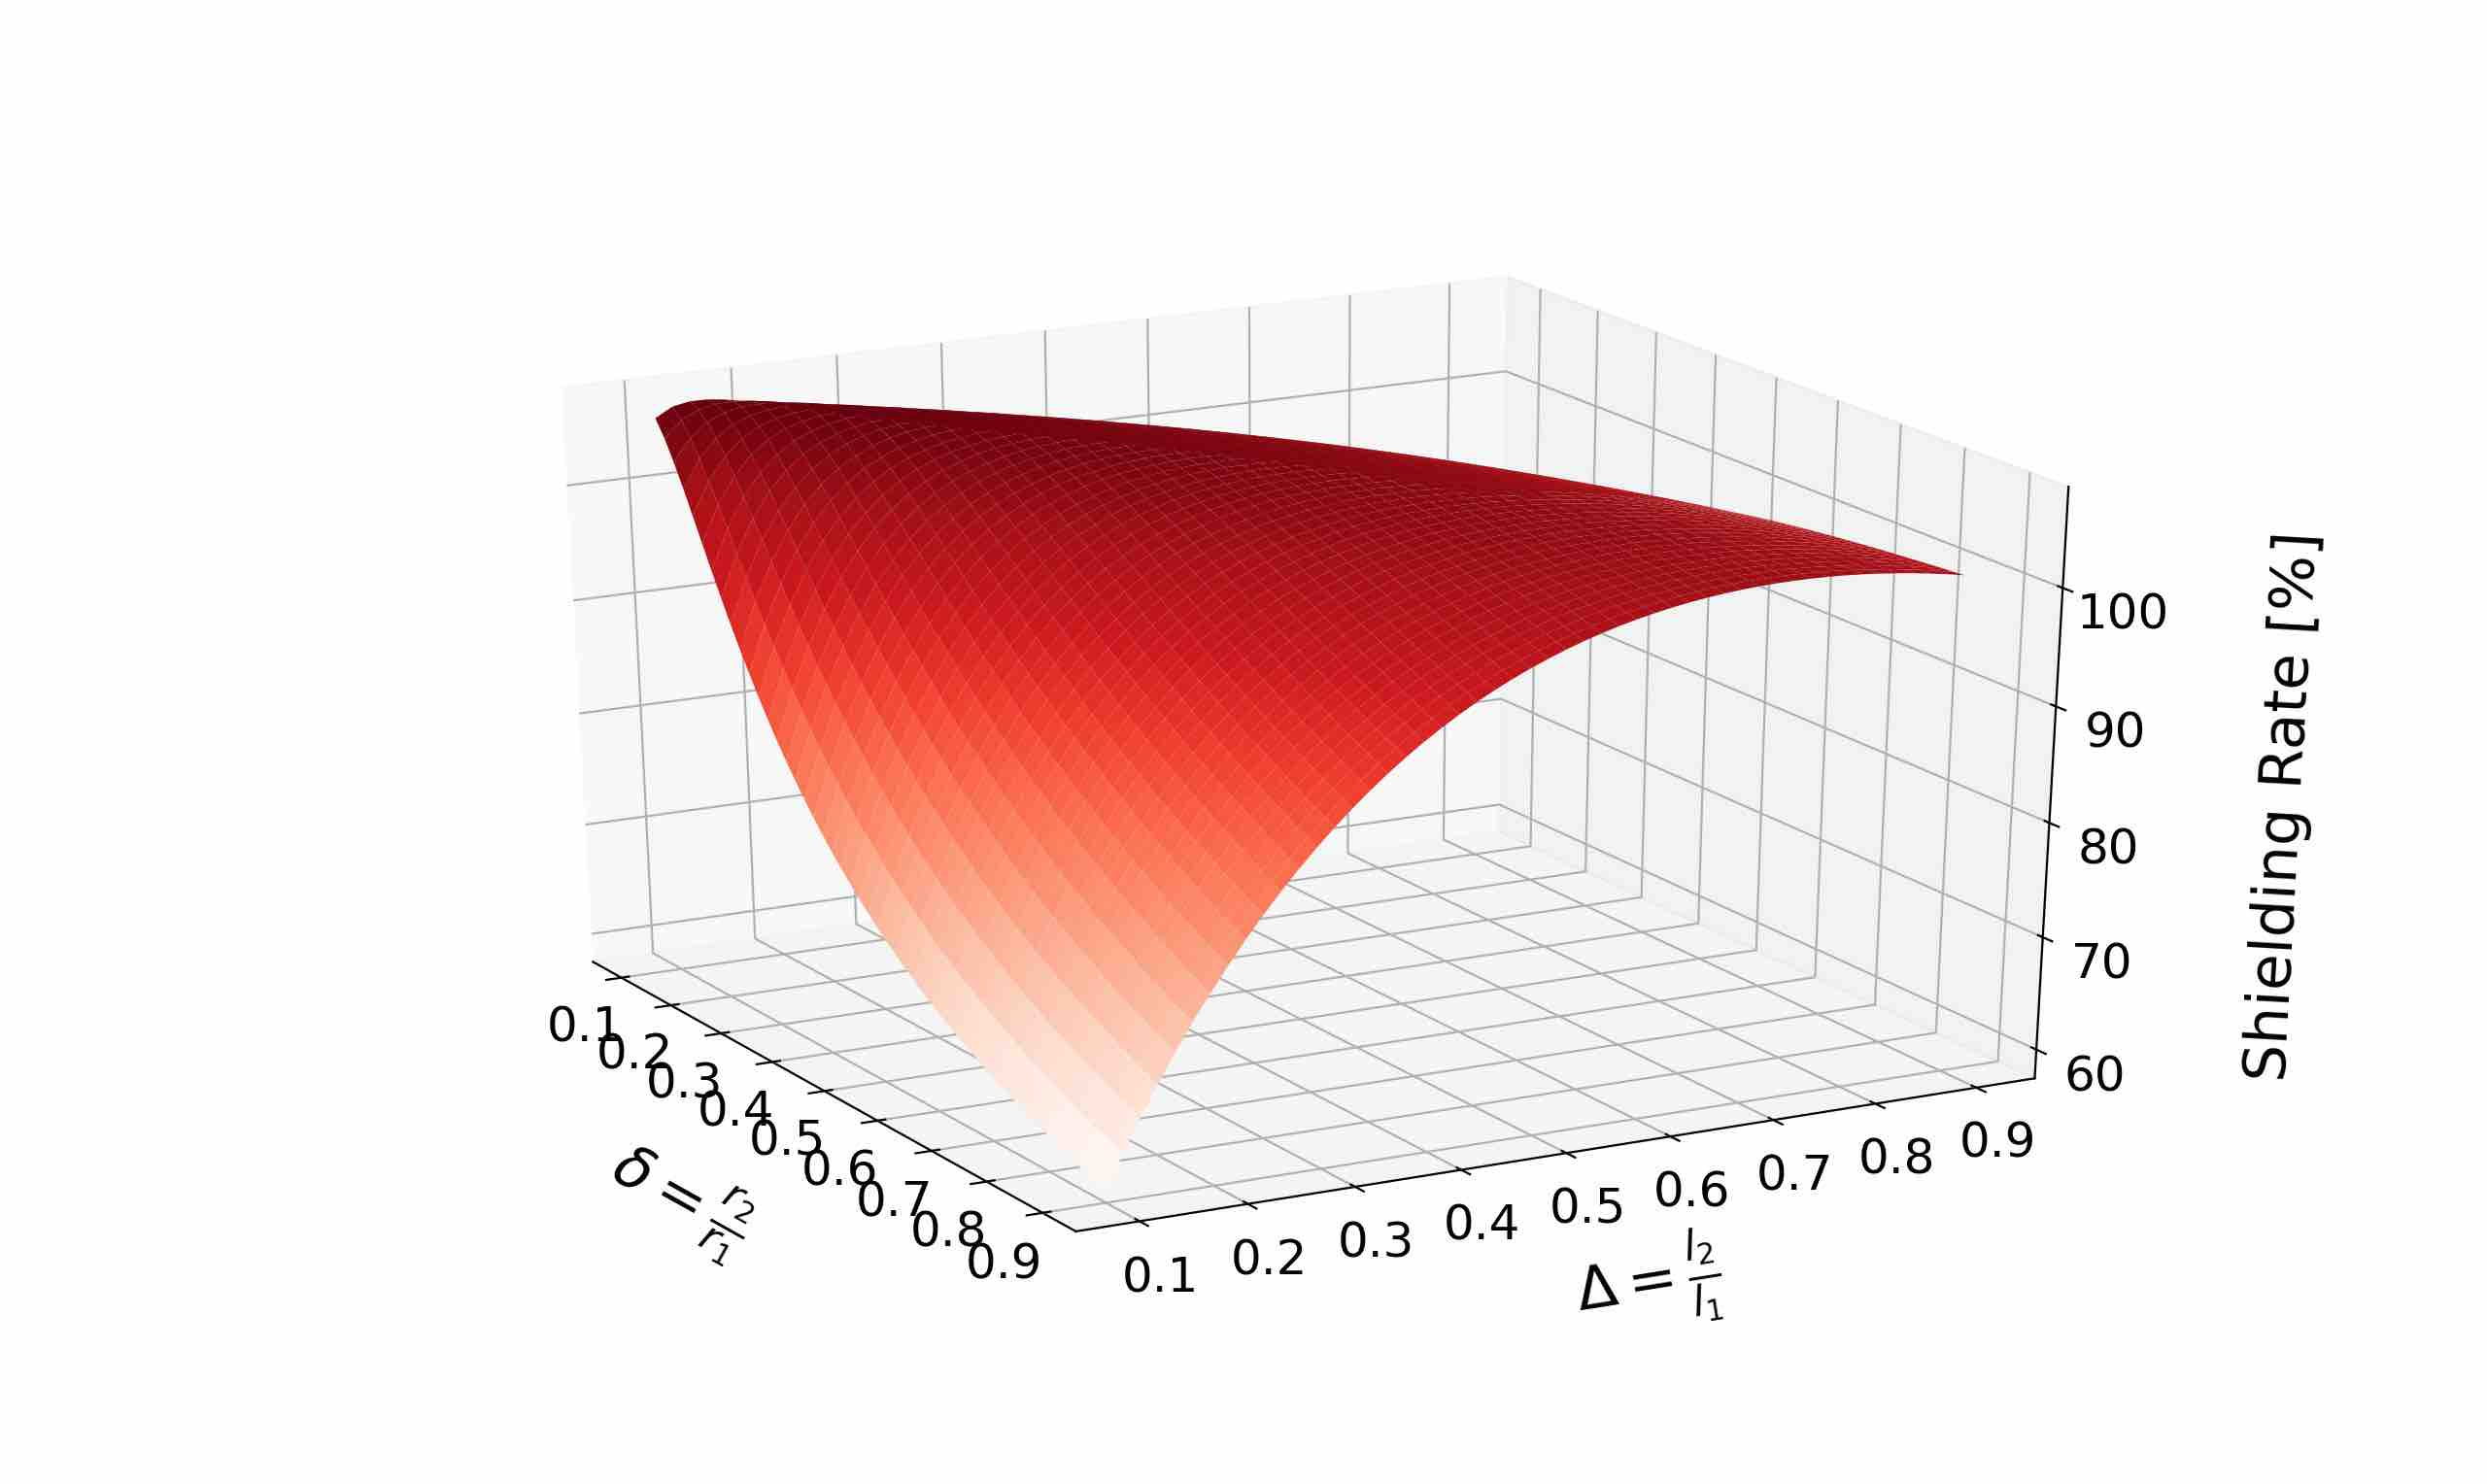
\includegraphics[width=17cm, bb=9 9 900 550]{./section3Effectiveness/simulatedShieldingRates3D2.JPEG}
  \caption{Simulated shielding rates with different $r_2, l_2$.}
  \label{fig:3D2}
\end{figure}
\begin{figure}[H]
  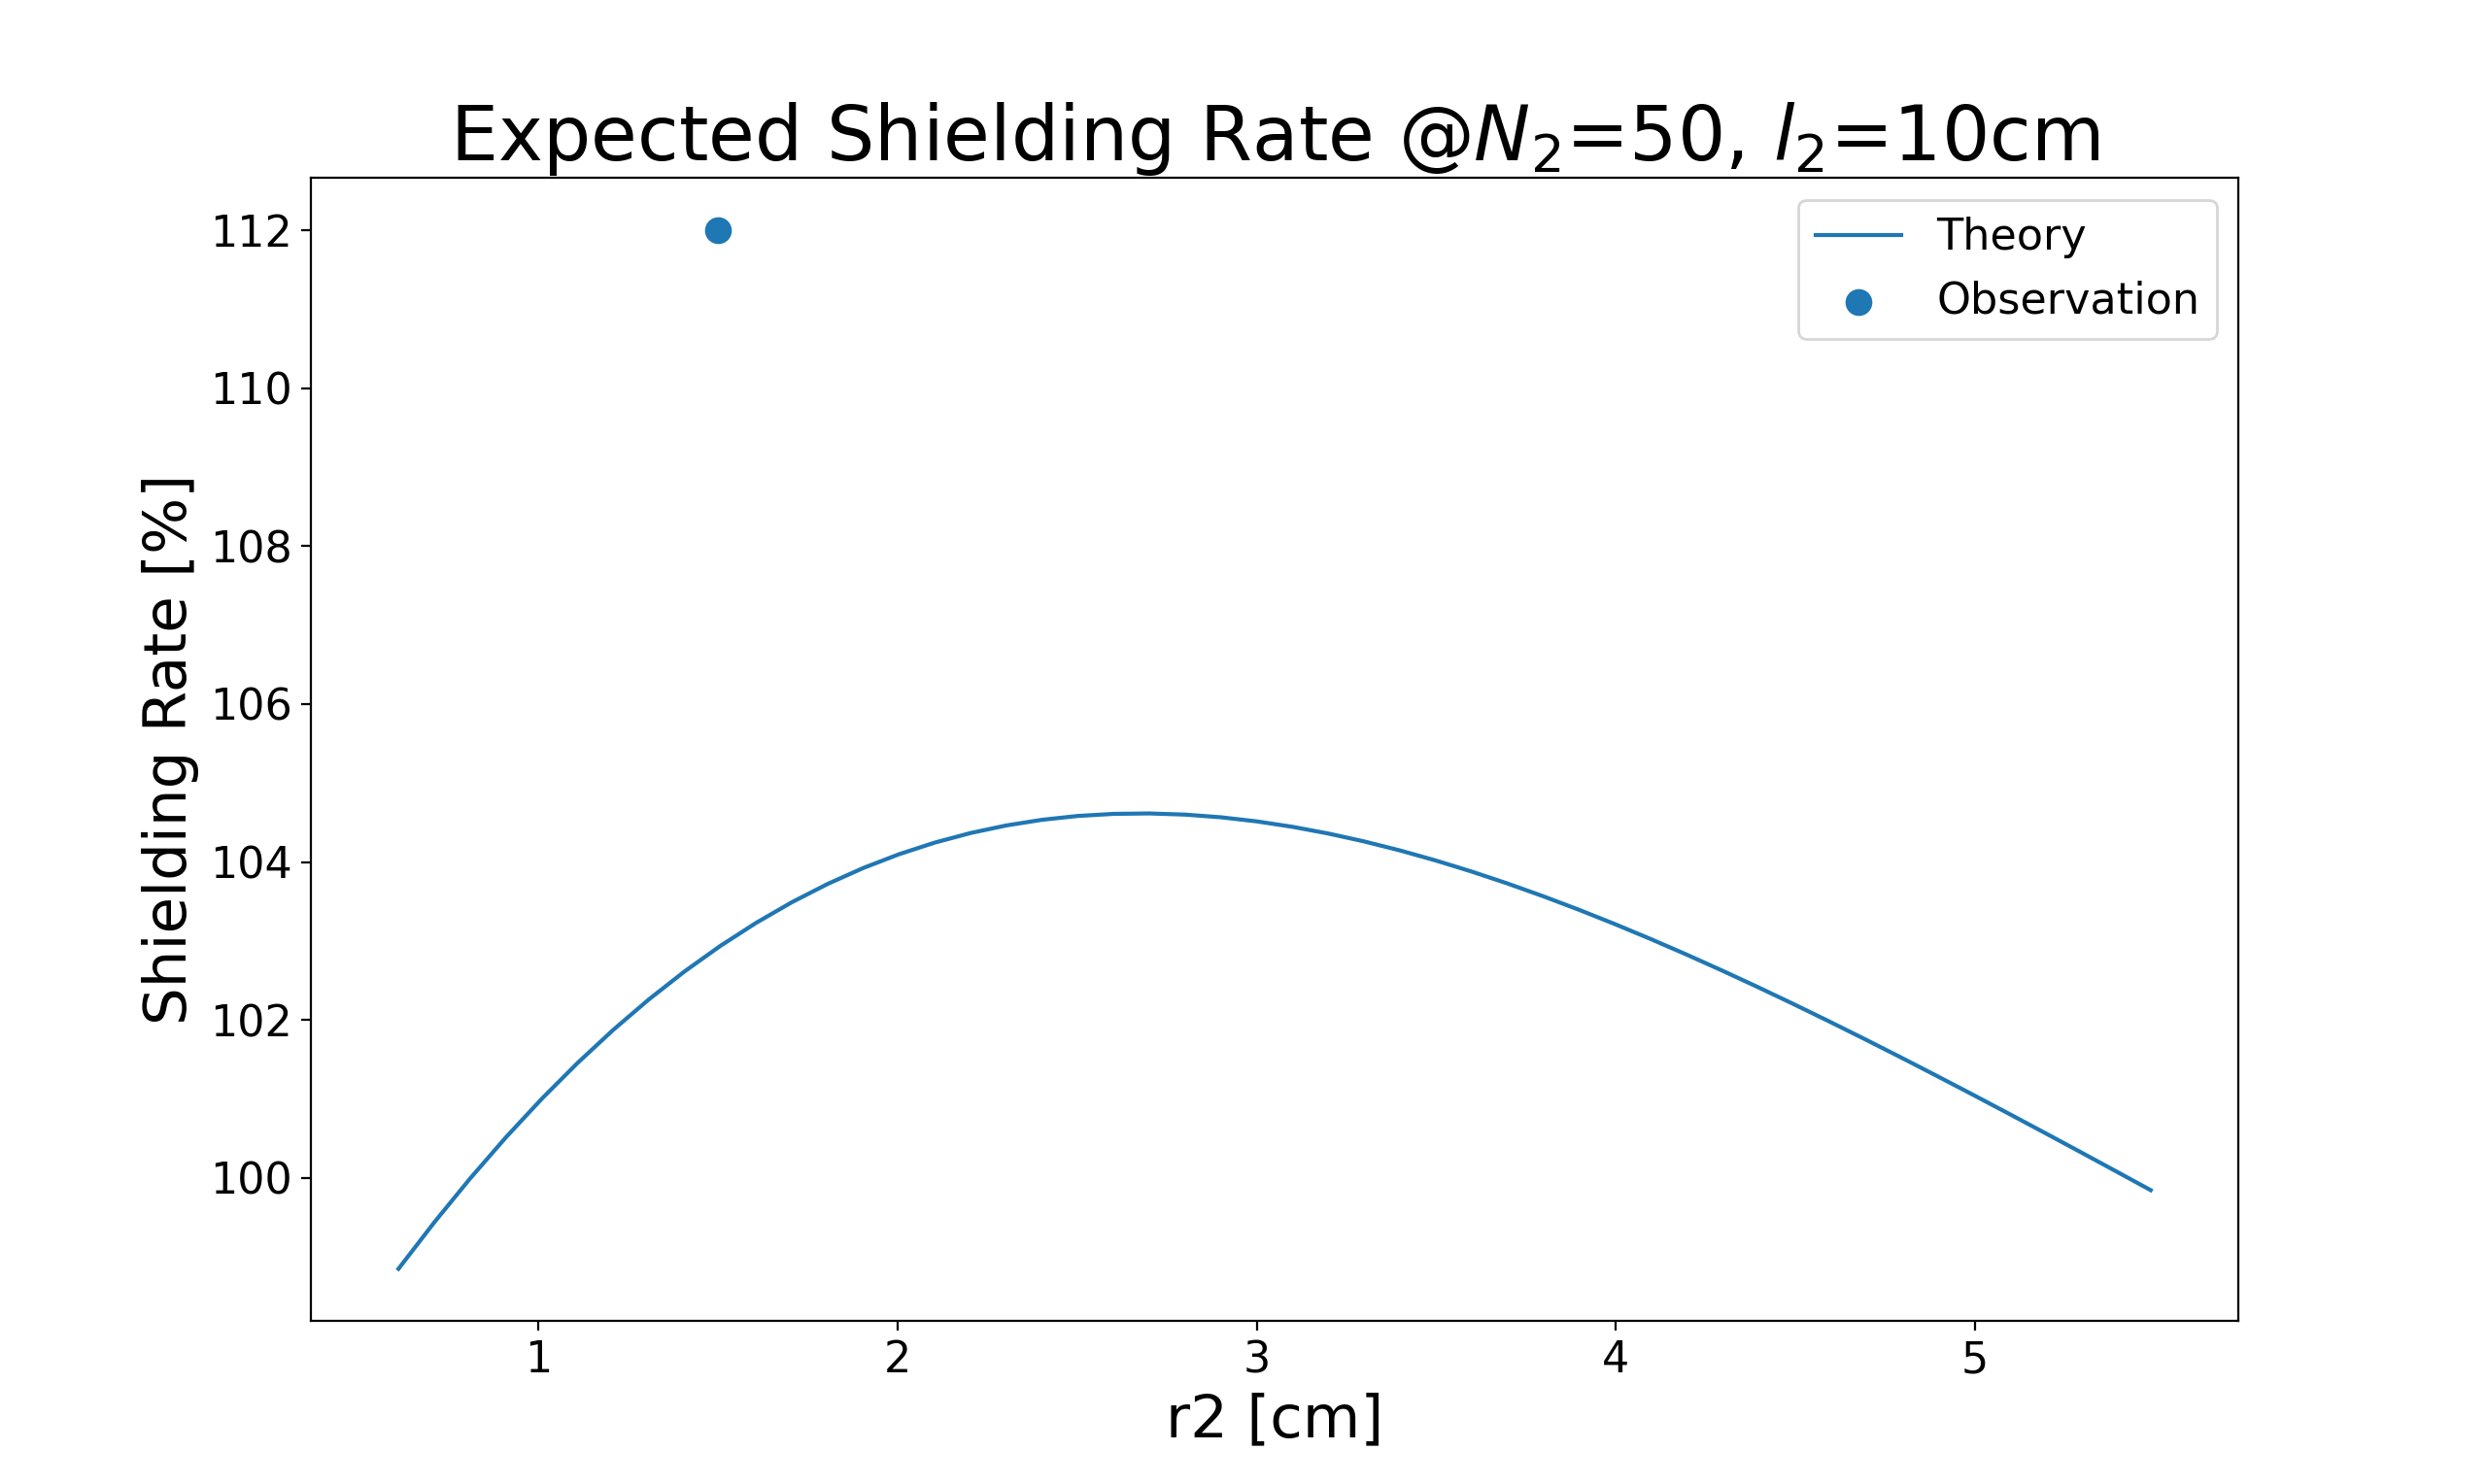
\includegraphics[width=17cm, bb=9 9 900 500]{./section3Effectiveness/simulatedShieldingRates2.png}
  \caption{Simulated and observed shielding rates with fixed $l_2 = 10$[cm], $N_2 = 50$, varied $r_2$.}
  \label{fig:overshielding}
\end{figure}

From Fig. \ref{fig:simulatedShieldingRates3D1} and \ref{fig:simulatedShieldingRates3D2},
2 notable points can be observed:
\begin{enumerate}
  \item As described, to achieve high shielding rates one must have the inner/outer coil aspect ratio falls into the right zone.
  For example, coils with radius ratio $\delta = r_2/r_1 = 0.5$ and length ratio $\Delta = l_2/l_1 = 0.5$ hold a shielding rates near 100\%,
  while coils with radius ratio $\delta = r_2/r_1 = 0.9$ and length ratio $\Delta = l_2/l_1 = 0.1$ only shows a poor performance around 70\%.
  \item It is possible for the central shielding rates to exceed 100\%.
  In Fig. \ref{fig:overshielding}, we have plotted the cross section at $l_2 = 0.5$ and $r_2 = 0.2\sim0.6$ out of Fig. \ref{fig:simulatedShieldingRates3D1} into a 2D diagram.
  In which, the simulated and experimental results both show shielding rates over 100\%.
\end{enumerate}

To explain this overshielding phenomenen, let us focus on how the inner current is induced.
From Faraday's law, electrical fields, or electrical currents if in conductive materials,
will be induced according to the magnetic field time variation ACROSS the surface.
This law is often described as the following equation, in integral form.
\begin{equation}
  \oint_{C} rot\mathbf{E}d\mathbf{r} = -\iint_{S}\frac{\partial B}{\partial t}d\mathbf{S}
\end{equation}
For a solenoid coil, the magnitude of the induced current is decided by the magnetic flux flow through the whole internal space.
Since Faraday's low only requires the magnetic field to balance in the entire internal space,
for some part of the space it is possible that the magnetic field produced by the induced current exceeds the field produced by the imposed current.
Physicists may find it easier to understand by considering the phenomenen resulting from the principle of minimum potential energy.
Engineers can approach from the fact that a solenoid winding generates a denser fields in the centeral part.
Anyway, even though overshielding occurs, as long as the shielding rates wanders around 100\%,
the actual magnetic field approaches zero.


\subsubsection{Method}
To testify the shielding rates, a series of experiments have been conducted useing the equipment introducd in section 3.1.
In this section, since the shielding rate is hard to measured under a DC condition,
we have chosen the imposed currents to be sin waves.
In this way, the induced currents on the internal coil would alse be sin waves,
from which the shielding effects can be measured easily from the magnitude.
To improve the accuracy, we have recorded 100 waves for each point, and measured the magnitude before they were averaged.
The procedure of our experiments is shown as following.
\begin{enumerate}
  \item Set the internal superconductor coil, and coil by liquid Nitrogen.
  \item Impose sin wave current continuously at specific magnitude and frequency.
  \item Measure the magnetic field variation in time domain, until data containing 100 wave lengths long are recorded.
  \item Transfer the measured magnetic field data into frequency domain data using fourier transform module provided by numpy.
  \item Take the magnitude at the certain imposed frequency and devided by the coefficient of the hall sensor,
  which is $89.34$ [$\mu$V/mT] in our experiments,
  to transfer the voltage data into $B$ field data.
  (Ensure the magnitude should be the maximum among the frequency domain data).
  This is taken as the measured $B$ field with shielding, at the certain position.
  \item If the $B$ field data along certain axis is need, then move to the next position and repeat from step 1.
  \item After the $B$ fields with shielding are recorded, remove the internal superconductor coil,
  and measure the $B$ fields along the same positions.
  Theese are taken as the measured $B$ field without shielding.
  Note that through the entire measuring experiments, the equipment is soaked in liquid Nitrogen.
\end{enumerate}
A 2 turn superconductive solenoid coil is used as the internal coil, while the external copper coil remains the same.
Parameters of this experiment is shown in Tab. \ref{tab:shieldingRateExpParameters}
\begin{table}[H]
  \centering
  \caption{Specification and parameters used in the shielding experiment.}
  \label{tab:shieldingRateExpParameters}
  \begin{tabular}{cccc}\hline\hline
    Parameter & Internal Coil1 & External Coil \\
    Diameter [cm] & 3.0 & 14\\
    Length [cm] & 10 & 20 \\
    Turns & 50 & 40 \\
    Critical Current $I_C$ [A] & 30 & Copper \\
    Width of Superconductor Tape & 12 & -\\\hline\hline
  \end{tabular}
\end{table}


\subsubsection{Result and Discussion}
The result of shielding rate measurement along the z axis is shown in Fig. \ref{fig:shieldingAbilityMeasuredBs}, and Fig. \ref{fig:shieldingAbilityMeasuredShieldingRates}.

\begin{figure}[H]
  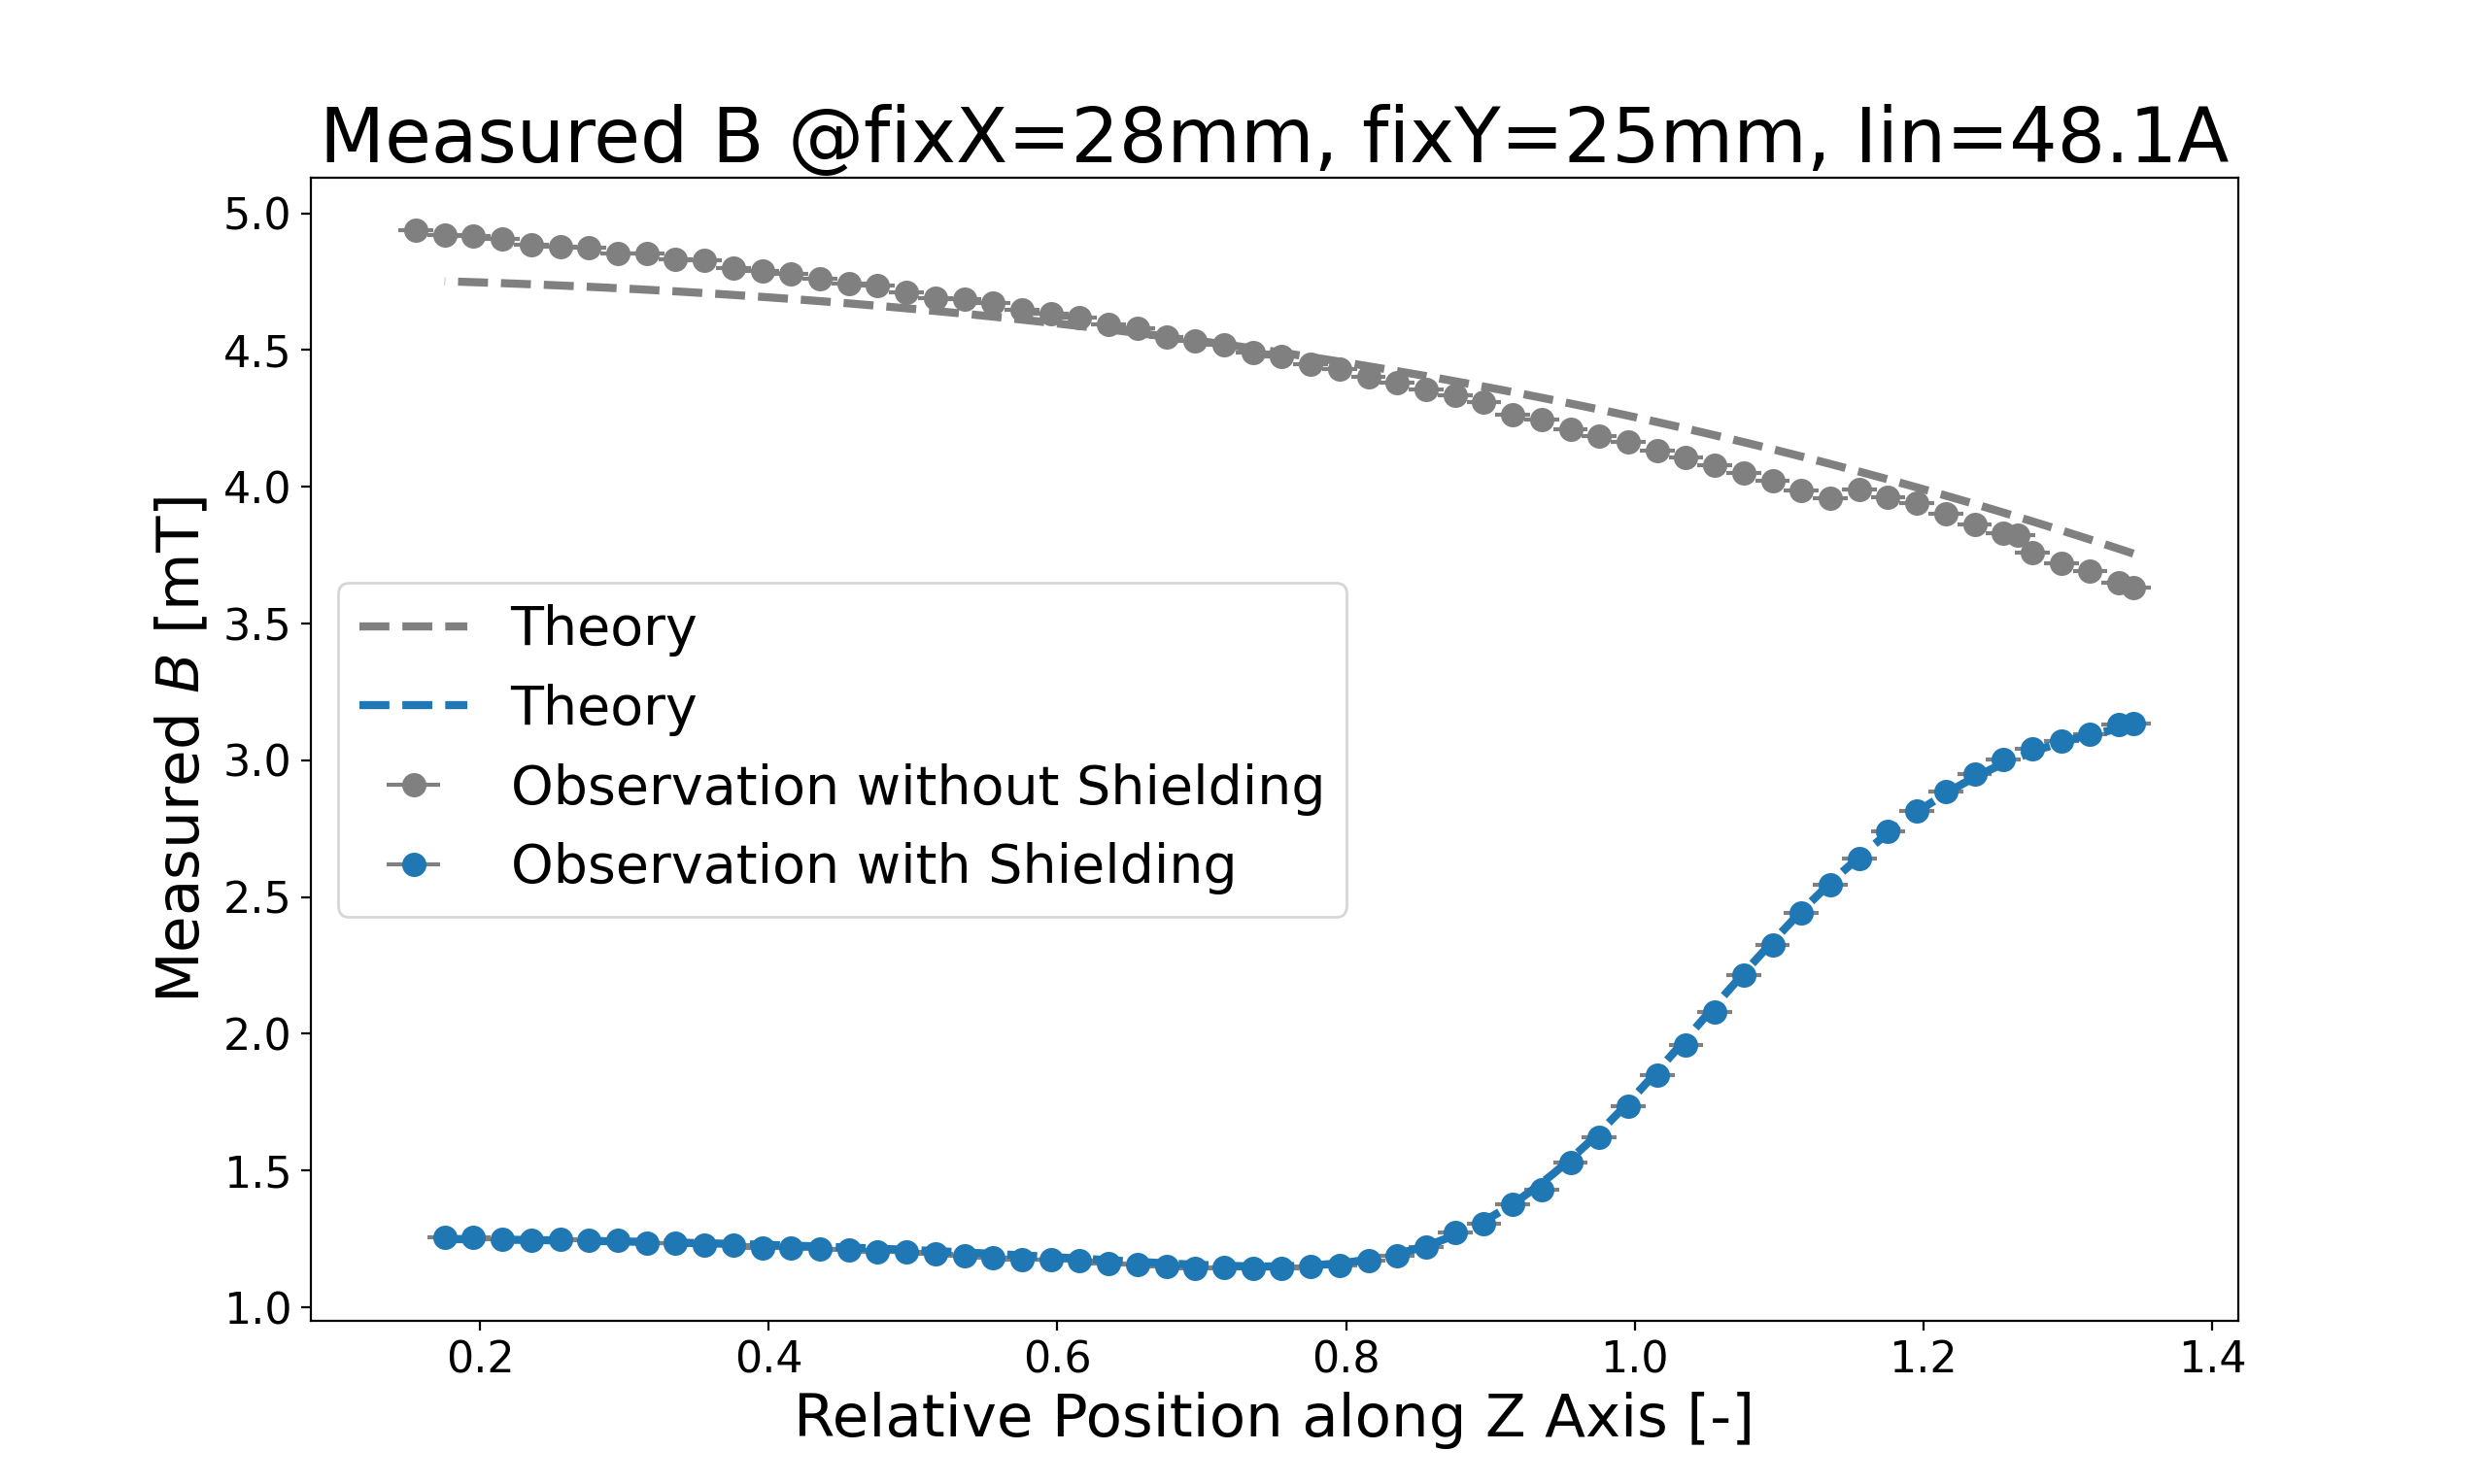
\includegraphics[width=17cm, bb=9 9 900 520]{./section3Effectiveness/measuredBsSolenoid.png}
  \caption{Measured magnitude $\mathrm{abs}(B)$ along the Z axis.}
  \label{fig:shieldingAbilityMeasuredBs}
\end{figure}
\begin{figure}[H]
  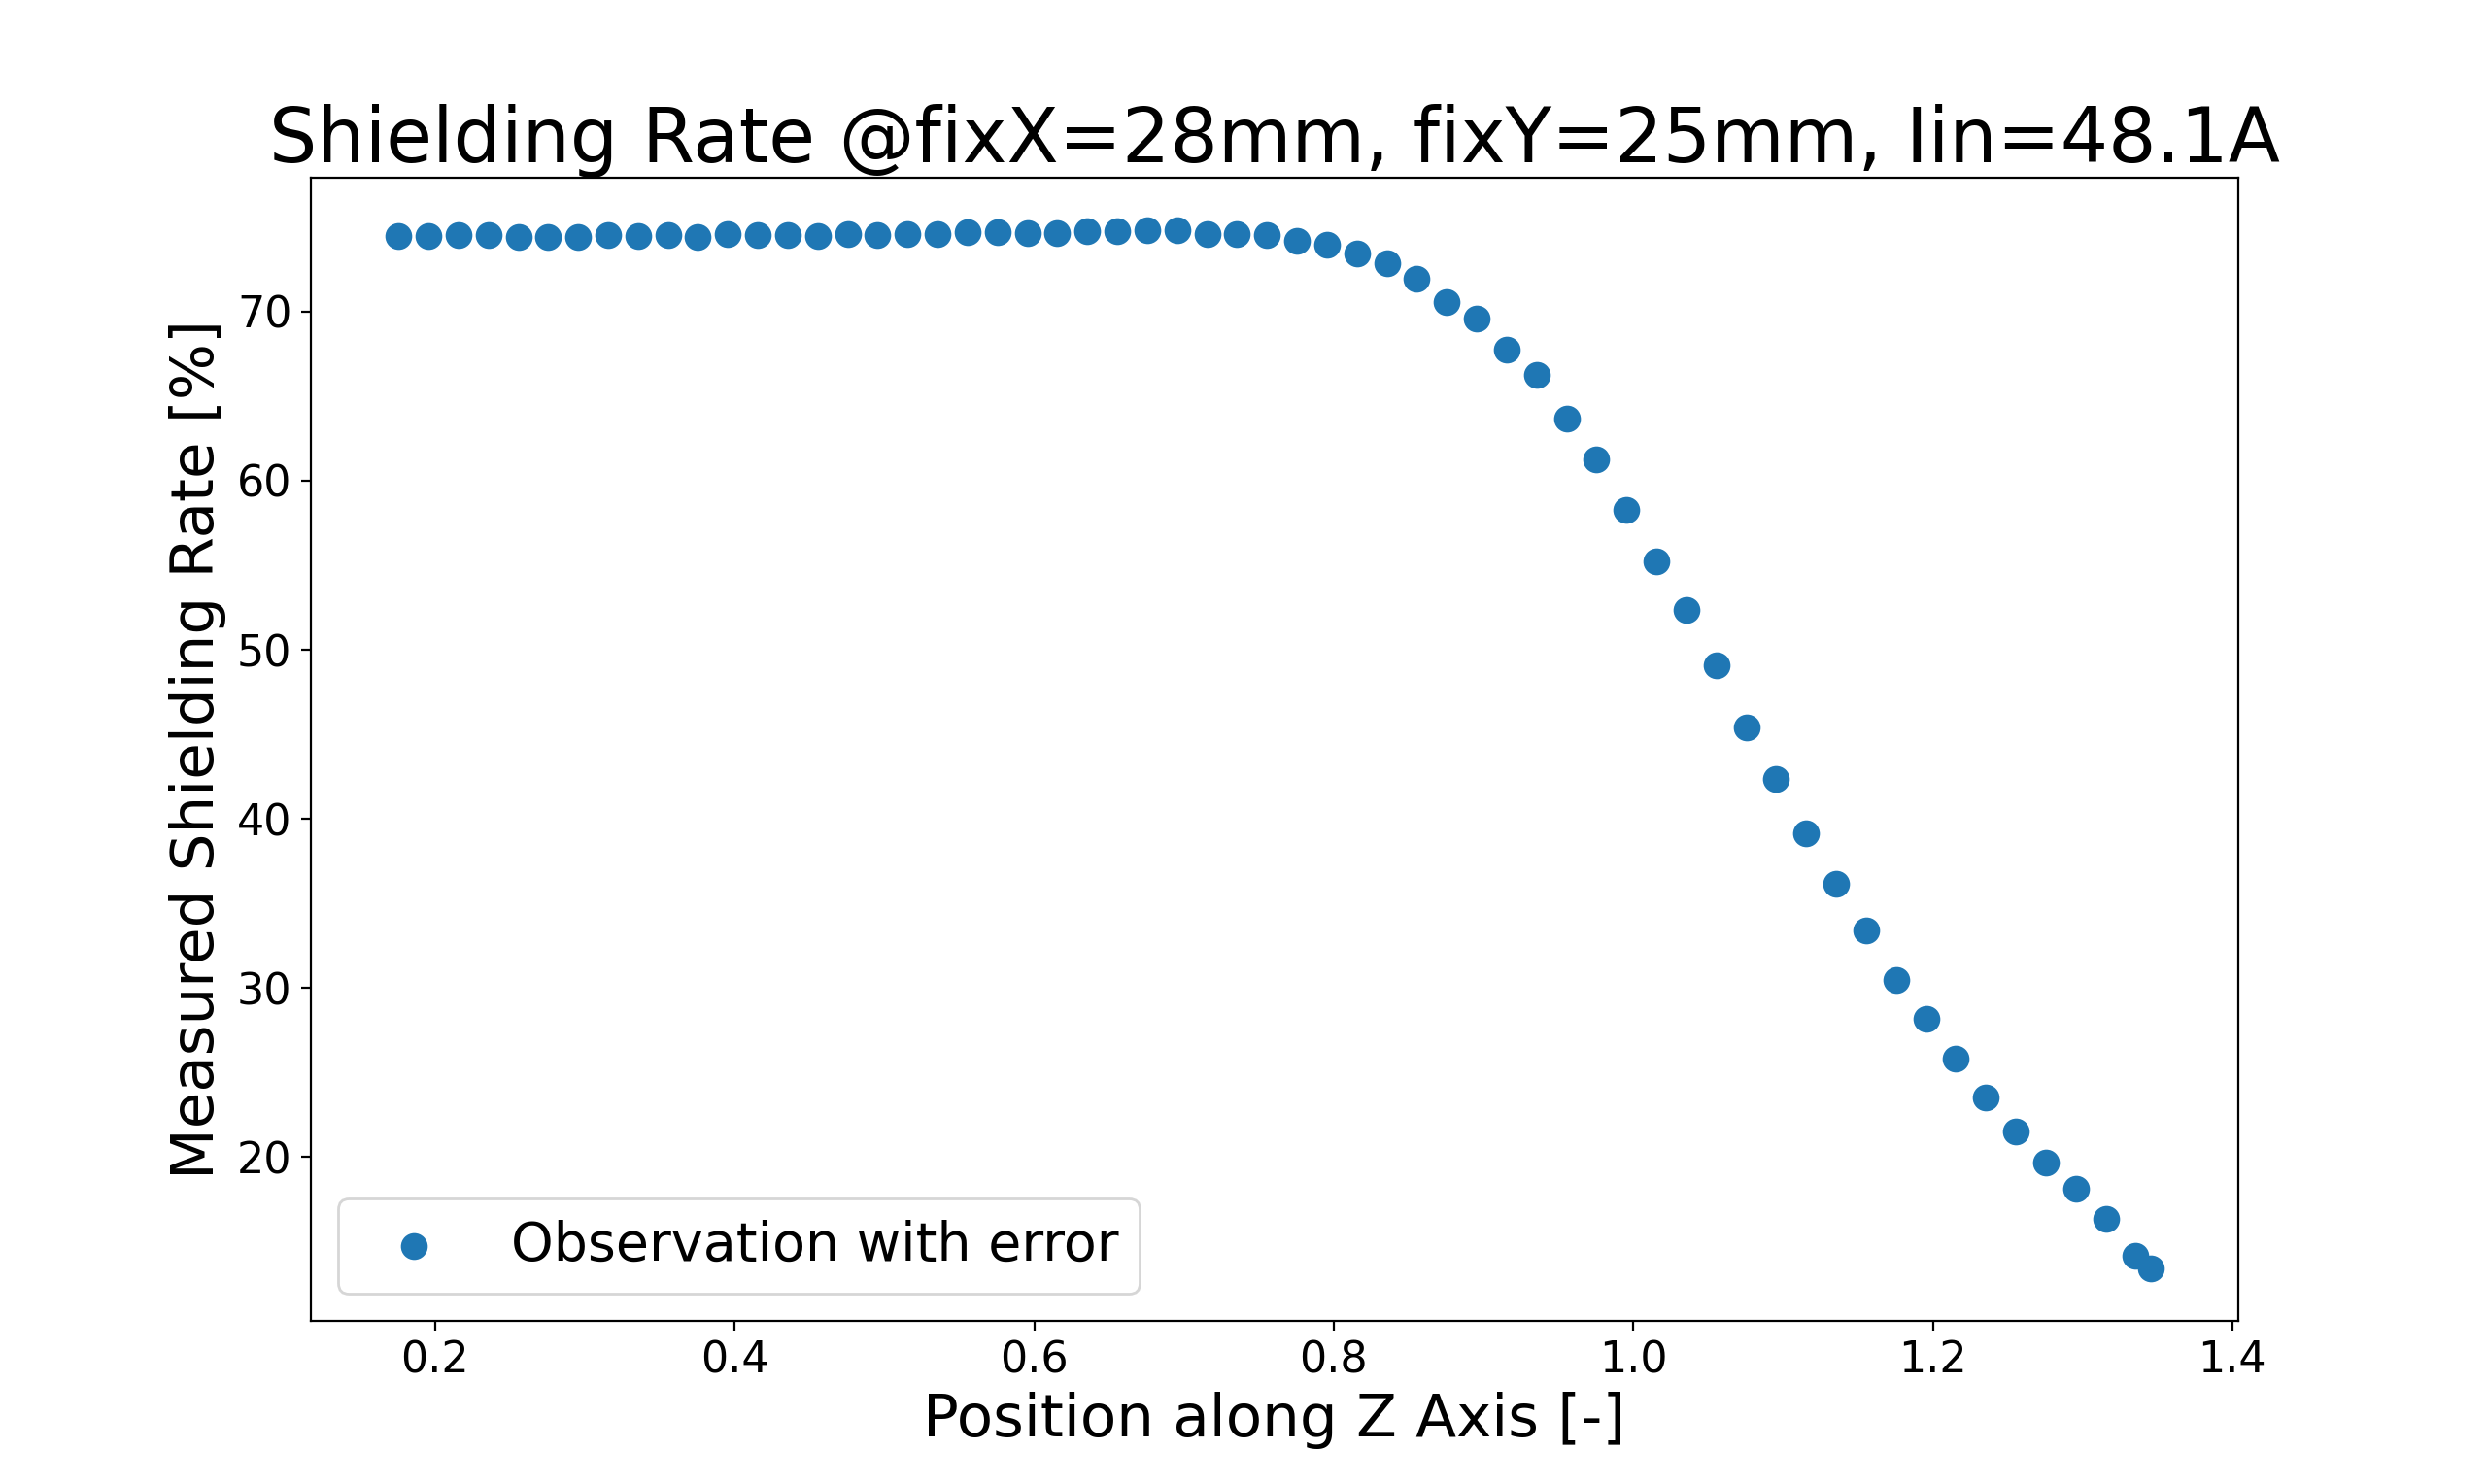
\includegraphics[width=17cm, bb=9 9 900 480]{./section3Effectiveness/measuredShieldingRatesSolenoid.png}
  \caption{The measured shielding rate and the expected shielding rates under ideal condition. The solid points are evaluated by $(1-B_{measured}/B_{imposed})$ directly from Fig.\ref{fig:measuredBSolenoid}, while the transparent points are evaluated by equation (4), along with the theoretical line.}
  \label{fig:shieldingAbilityMeasuredShieldingRates}
\end{figure}
In Fig. \ref{fig:shieldingAbilityMeasuredShieldingRates},
the solid points represent the measured $B$ fields along the z axis.
From which, the shielding rate reaches around 78\% inside the internal coil.
The outer the position gets, the lower the shielding rate goes.

The maximum shielding rate 78\% may seem low.
This is due to the coil being small, with low inductance and relatively high resistance.
According to equation (30) or (35), the shielding rate should be no concern with the impedance including $\omega L$ and $R$,
as shown below.
\begin{eqnarray}
  B(t) &=& C_1\cdot i_1(t) - C_2\cdot i_2(t)\nonumber\\
  &|& C_1 = \sum_{i=1}^{N1} \frac{\mu_0r_1^2}{2\left(r_1^2 + d_i^2\right)^{\frac{3}{2}}} \in \mathrm{constant}\nonumber\\
  &|& C_2 = \sum_{i=1}^{N2} \frac{\mu_0r_2^2}{2\left(r_2^2 + d_i^2\right)^{\frac{3}{2}}} \in \mathrm{constant}\nonumber\\
  &|& i_1(t) = I_1\sin(\omega t)\nonumber\\
  &|& i_2(t) = \frac{M}{L_2}I_1\sin(\omega t)\nonumber\\
  &=& \left(C_1I_1 - C_2\frac{MI_1}{L_2}\right)\sin(\omega t)|\omega L_2 \gg R_2\\
  Shielding Rate &=& \frac{C_2\cdot i_2(t)}{C1\cdot i_1(t)} = \frac{C_2}{C_1}\cdot\frac{M}{L_2}
\end{eqnarray}
However, if the $\omega L_2 \ll R_2$ doesn't hold, which means the resistance of the internal coil is not neglectable,
the induced current would become
\begin{eqnarray}
  i_2(t) &=& \frac{j\omega M}{j\omega L_2 + R_2}\cdot I_1\sin(\omega t)\nonumber\\
  &=& \frac{1}{\sqrt{1+\left(\frac{R_2}{\omega L_2}\right)^2}}\cdot \frac{M}{L_2}I_1\sin(\omega t + \theta)\\
  &|& \theta = \tan^{-1}(\frac{R_2}{\omega L_2})\nonumber
\end{eqnarray}
where $j$ denotes the imaginary unit, $M$ denote the mutual inductance of the inner-outer coils,
$L_2$ denotes the inductance of the inner coil.
Mark that the transient term is emitted here for convenience.
With equation (39), it is obvious that the magnitude of the induced current $i_2(t)$ is multiplied by
$\frac{1}{\sqrt{1+(\omega L_2)^2}} < 1$ and the phase of which is delayed by $\theta > 0$,
which indicates a weaker induce current as well as a weaker magnetic shielding ability.
Accordingly, the magnetic field $B$ distribution along Z axis can be denoted as equation (40) and the shielding rate can be derived to be equation (41).
\begin{eqnarray}
  B(t) &=& C_1I_1\sin(\omega t) - \frac{C_2}{\sqrt{1+\left(\frac{R_2}{\omega L_2}\right)^2}}\cdot \frac{M}{L_2}I_1\sin(\omega t + \theta)\nonumber\\
  &|& \theta = \tan^{-1}(\frac{R_2}{\omega L_2})\nonumber\\
  &=& \sqrt{a^2 - 2ab\cos(\theta) + b^2}\cdot\sin(\omega t - \phi)\\
  &|& \phi = \tan^{-1}\left(\frac{b\sin(\theta)}{a-b\cos(\theta)}\right)\nonumber\\
  &|& a = C_1I_1 \in \mathrm{constant}\nonumber\\
  &|& b = \frac{M/L_2}{\sqrt{1+\left(\frac{R_2}{\omega L_2}\right)^2}}C_2I_1 \in \mathrm{constant}\nonumber
\end{eqnarray}
\begin{eqnarray}
  Shielding Rate = \frac{C_2}{C_1}\cdot\frac{M}{L_2} = \frac{b}{a}\cdot\sqrt{1+\tan^2\left(\theta\right)}
\end{eqnarray}
The parameter $a, b, \theta, \phi$ in equation (39), (40) can be measured directly, from which the shielding rate can be evaluated.
For instance, example plots of equation (40) with different $\theta$, namely, different $\omega L_2$ and $R_2$,
are shown in Fig.\ref{fig:0.1theta} and Fig.\ref{fig:14theta}
\begin{figure}[H]
  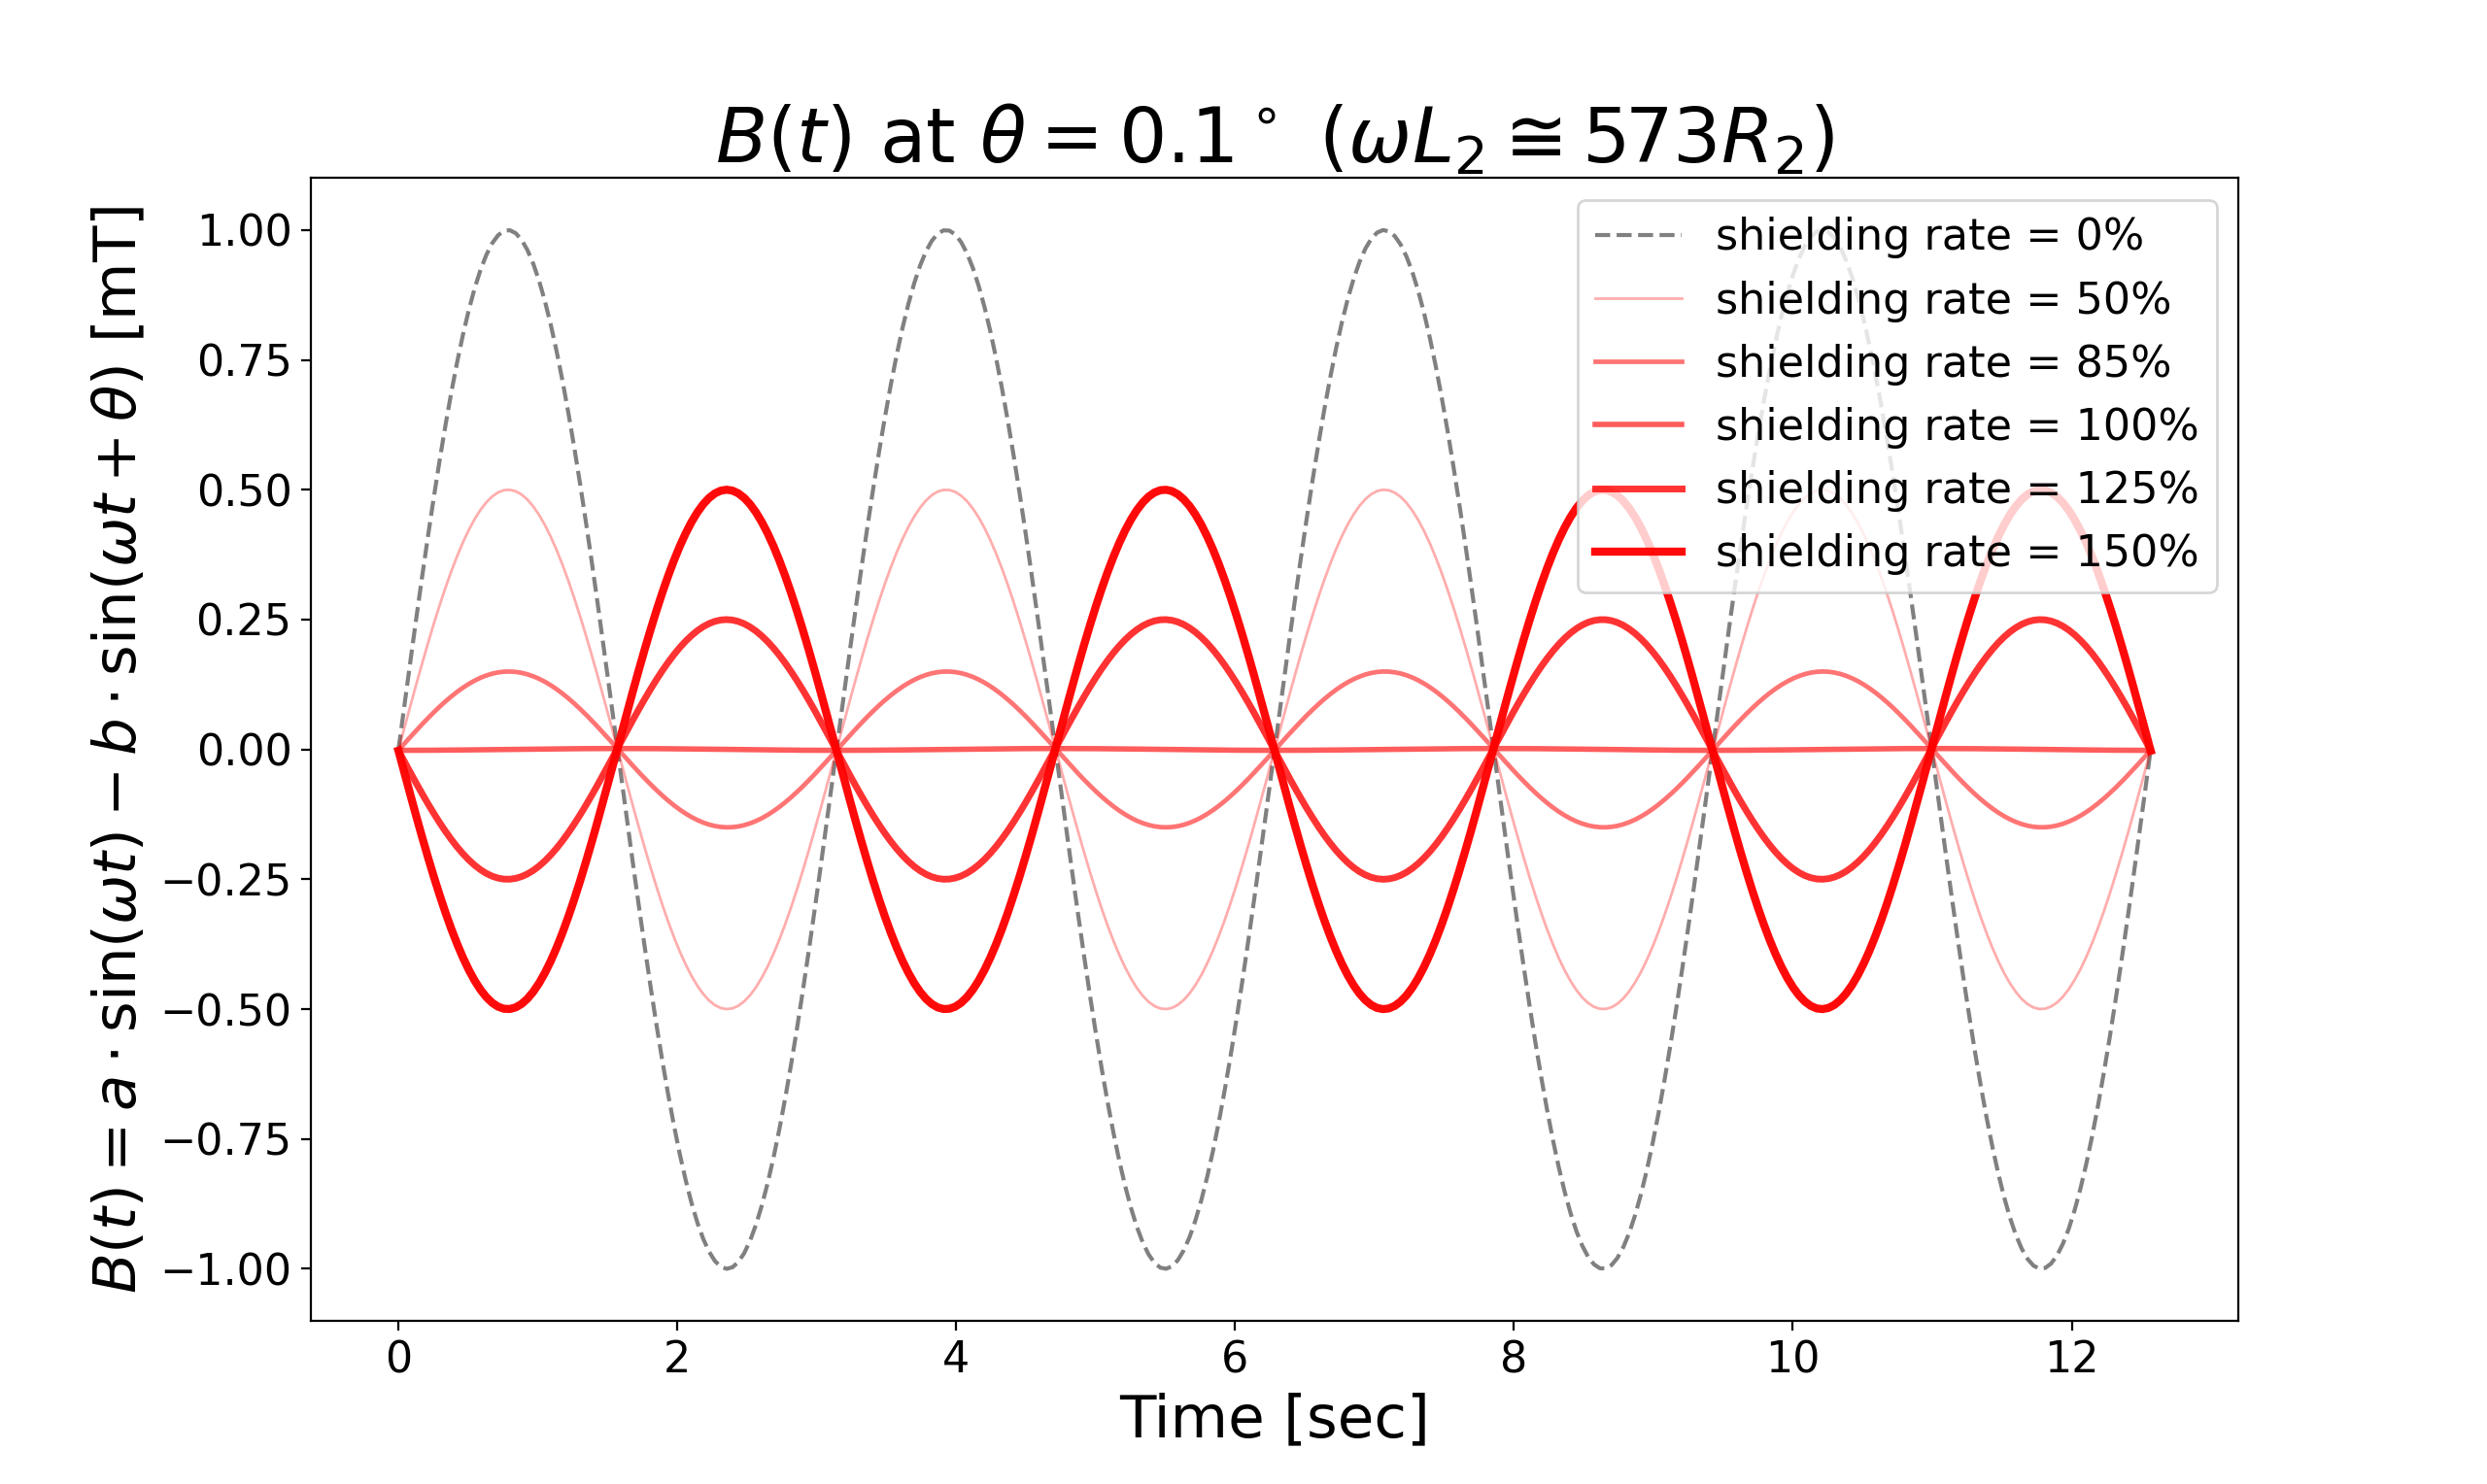
\includegraphics[width=17cm, bb=9 9 900 550]{./section3Effectiveness/sinTestAt0.1deg.png}
  \caption{Simulated $B$ using equation (40) with $\theta = 0.1^\circ$ ($\omega L_2 \cong 573R_2$).}
  \label{fig:0.1theta}
\end{figure}
\begin{figure}[H]
  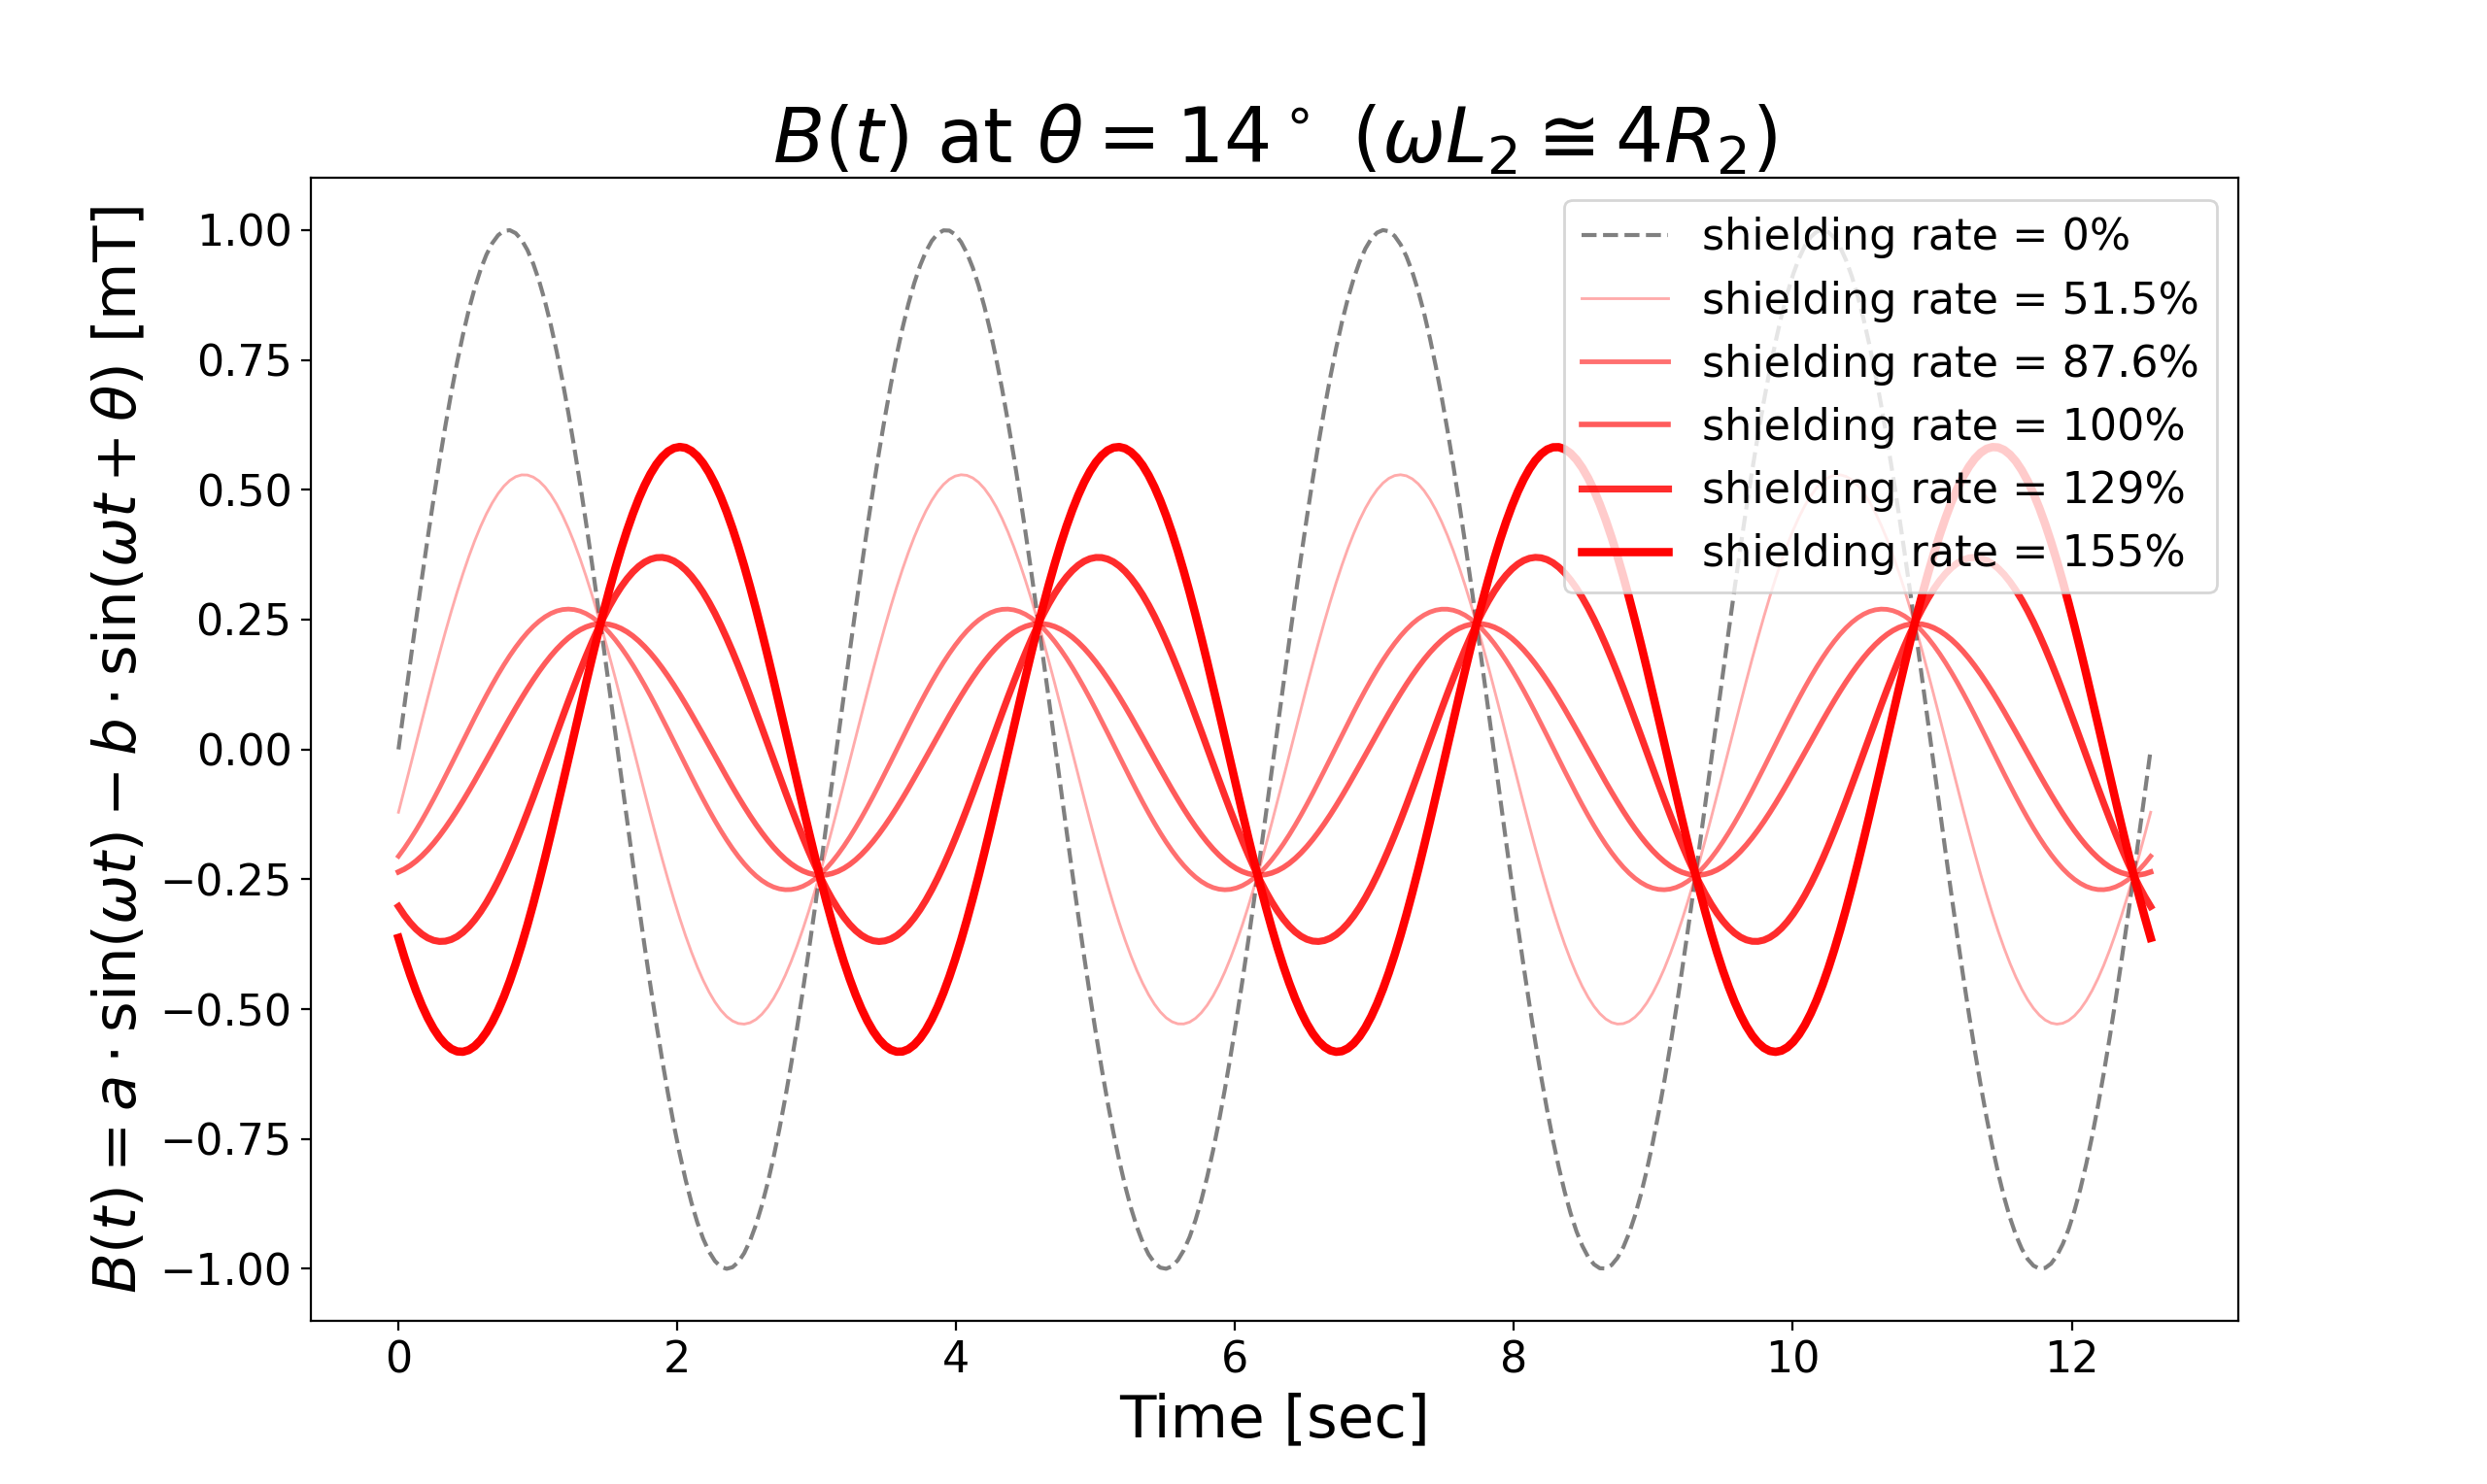
\includegraphics[width=17cm, bb=9 9 900 490]{./section3Effectiveness/sinTestAt14deg.png}
  \caption{Simulated $B$ using equation (40) with $\theta = 14^\circ$ ($\omega L_2 \cong 4R_2$).}
  \label{fig:14theta}
\end{figure}
From the above plots, in the condition that the induced current $i_2$ is delayed by $\theta$,
even if the shielding rate matches 100\% residual magnetic field $B$ remains none zero.

To sum it up, in a relatively small coil model with over shielding happened, the shielding rate would be small compared to a relatively large scale model.
Expand the measured $B$ data to a $\omega L \gg R$ condition raises the transparent points shown in Fig. \ref{fig:shieldingAbilityMeasuredShieldingRates}.
From which, shielding rates inside the coil around 100\% can be expected.
This expectation is close to the result of simulation, shown in the same graph by a transparent line.
It indicates that in a full scale model, a shielding rate at least 95\% is achievable,
which is suitable working as a magnetic field shielding system.


\subsubsection{Conclusion}
In this section, we have measured the shielding rates along the z axis on a scaled down model.
Although the measured shielding rate shows a peak of about 78\%,
in full scale models it can be epected to be over 95\%.
95\% shielding rate means the field inside the internal coil may be down to 50 mT when the external field is 1 T,
which is small enough for normal electrical equipments to work.
Needless to say, if more shielding is needed,
this system is free to be combined with any general magnetic field shielding system, such as the ones using normal ferromagnets.


\newpage
\subsection{Effect of Ferromagnets}
To avoid the weaking of the field near the shielding system,
we have proposed that inserting ferromagnets on the top of the superconductor coil,
expecting strong magnetization to reinceforce the field.
In this section, we have conducted a series of experiments to confirm the effect of ferromagnet.
As before, the purpose, the theory, the method and the result is shown in the following sections.

\subsubsection{Purpose}
The purpose of this experiment is to proof that ferromagnets do increase the field near the edge of the superconductor coil.

\subsubsection{Theory}
In section 2.3 we have already introduced the physical foundation of the ferromagnetism,
which is,
strong magnetization $M$ in a ferromagnet would be induced even though the imposed field is weak.
The equation
\begin{equation}
  B = M + \mu_0 H
\end{equation}
must hold.
Although the direction of $M$ is not always strictly identical with $B$ and $H$,
the direction is almost the same.
In the following paragraphs, further discussion about the $B$ and $M$ field is denoted,
approaching from the vector potential.

Consider an Electromagnetic Induction type magnetic cloak model, with curve ferromagnets placed in the upper and lower edge,
as shown in Fig. \ref{fig:EIMC_modelWithFM}.
Note that only the internal coil and ferromagnet are plotted,
the external coil are ommited here.
\begin{figure}[H]
  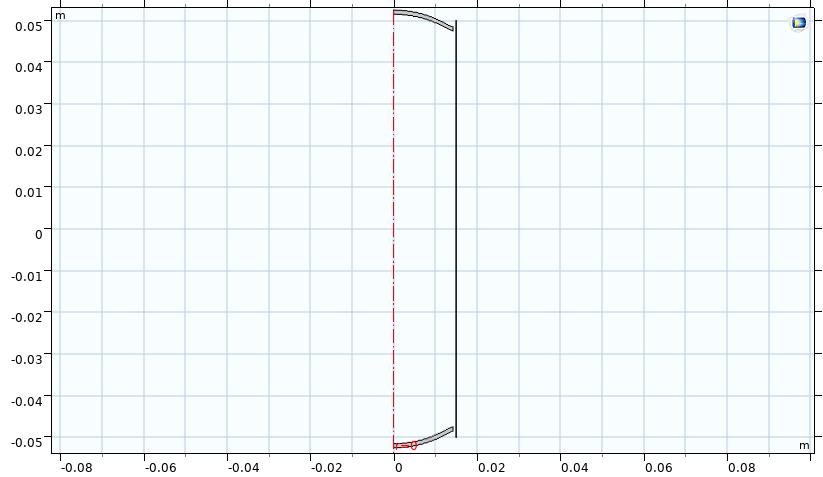
\includegraphics[width=17cm, bb=9 9 900 550]{./section3Effectiveness/plannedFM2Structure.png}
  \caption{The axisymmetric model used in our simulation. Note that only the inner coil is plotted here.}
  \label{fig:EIMC_modelWithFM}
\end{figure}
A cylindrical coordinates $(\rho, \phi, z)$ is used in this model,
in which the vector potential $\mathbf{A}_p(\rho, 0, z)$ at point $p(\rho, 0, z)$ is the combination of
the potential generated by the coil $\mathbf{A}_{coil}$,
the potential generated by the outer surface of the upper magnet $\mathbf{A}_{magUpperSurface}$,
and the potential generated by the inner surface of the upper magnet $\mathbf{A}_{magLowerSurface}$,
\begin{eqnarray}
  \mathbf{A}_p(\rho, 0, z) &=& \mathbf{A}_{coil} + \mathbf{A}_{magUpperSurface} + \mathbf{A}_{magLowerSurface}\\\nonumber
  &=& \sum_{i=1}^{N}\frac{\mu_0I_1}{\pi k_c}\sqrt{\frac{\rho'_c}{\rho}}\left((1-\frac{1}{2}k_c^2)K(k_c) - E(k_c)\right)\\\nonumber
  &+& \int_{Z_{LO}}^{Z_{UO}}dz'_{mO}\cdot\frac{\mu_0k_{\phi'}}{\pi k_{mO}}\sqrt{\frac{\rho'_{mO}(z'_{mO})}{\rho}}\left((1-\frac{1}{2}k_{mO}^2)K(k_{mO}) - E(k_{mO})\right)\\\nonumber
  &+& \int_{Z_{LI}}^{Z_{UI}}dz'_{mI}\cdot\frac{\mu_0k_{\phi'}}{\pi k_{mI}}\sqrt{\frac{\rho'_{mI}(z'_{mI})}{\rho}}\left((1-\frac{1}{2}k_{mI}^2)K(k_{mI}) - E(k_{mI})\right)\mathbf{e}_{\phi}\\\nonumber
  &,& K(k) = \mathrm{TheFirstKindCompleteEllipticIntegralWithModulus} k\\\nonumber
  &,& E(k) = \mathrm{TheSecondKindCompleteEllipticIntegralWithModulus} k\\\nonumber
  &,& k_c = \sqrt{\frac{4\rho\rho'_c}{(\rho+\rho'_c)^2+(z-z'_{ci})^2}}\\\nonumber
  &,& k_{\phi'} = (\mathbf{M}\times\mathbf{n})_{\phi'}\\\nonumber
  &,& k_{mO} = \sqrt{\frac{4\rho\rho'_c}{(\rho+\rho'_c)^2+(z-z'_{mO})^2}}\\\nonumber
  &,& k_{mI} = \sqrt{\frac{4\rho\rho'_c}{(\rho+\rho'_c)^2+(z-z'_{mI})^2}}\nonumber
\end{eqnarray}
where $\rho'_c$ represents the coil's radius,
$z'_{ci}$ represents the z position of the $i$th turn,
$z'_{mO}$ represents the z position of the outer magnet surface varying from $Z_{LO}$ to $Z_{UO}$,
$z'_{mI}$ represents the z position of the inner magnet surface varying from $Z_{LI}$ to $Z_{UI}$,
$\rho'_{mO}(z)$ represents the radius distribution of the outer magnet surface which is a function of $z'_{mO}$,
$\rho'_{mI}(z)$ represents the radius distribution of the inner magnet surface which is a function of $z'_{mI}$.
Mark that in equation (43) only the magnetization $\mathbf{M}$ and the induced current $I_1$ are variables,
once they are determined the vector potential can be solved directly.
However, even though we can solve the induced current term by Bio-Savart's law,
the magnetization terms are hard to solve.
Therefore, we have used the finite element method to solve it numerically.


\subsubsection{Method}
To measure the effect of ferromagnets, we have conducted a series of simulation and experiments.
Two internal coil models have been evaluated,
one with ferromagnets placed on the top and bottom edge of the superconductor coil,
another only the superconductor coil.
The superconductor coils here are not simple solenoid windings as the ones used in the previous sections,
but are windings with more turns near the edge and less turns at the central,
which we name it the "distributed coil".
The parameters of the equipments are shown in Tab. \ref{tab:distributedCoil},
and a photograph of the actual distributed coil windings is shown in Fig. \ref{fig:photoDistributedCoil}.
\begin{figure}[H]
  \includegraphics[width=9.5cm, bb=9 9 900 1500]{./section3Effectiveness/distributedCoil.png}
  \caption{The distributed coil under test.}
  \label{fig:photoDistributedCoil}
\end{figure}
\begin{table}[H]
  \centering
  \caption{Specification of the experiment.}
  \label{tab:distributedCoil}
  \begin{tabular}{cccc}\hline\hline
    Parameter & Distributed Coil with Ferromagnet & Distributed Coil without Ferromagnet & External Coil \\\hline
    Diameter [cm] & 3.0 & 3.0 & 14\\\hline
    Length [cm] & 10 & 10 & 20 \\\hline
    Turns & 50 & 50 & 40 \\\hline
    Critical Current $I_C$ [A] & 120 & 120 & Copper \\\hline
    Width of Superconductor Tape & 4 & 4 & -\\\hline\hline
  \end{tabular}
\end{table}

For the simulation,
we have used the finite element method provided by commercial software Comsol Multiphysics Inc. to solve the vector potential $A$ around the model,
and latter derived the magnetic field distribution from the potential field.
The external field we used is a model of MRI coils, of which the detail would be describe in chapter 5.
Since it is almost uniform within the internal space, it can be considered uniform field here.

For the experiment,
we have made the two coils as denoted above, with one of which covered by a $0.6$ mm ferit sheet.
Due to the central part of the windings being sparse,
we have also placed a layer of ferit sheet on the inner wall of the FM model to see if the it can perform any shielding effect to increase the shielding effect.
The procedure of the experiment is the same as the one conducted in the previous section,
with AC imposed fields and the axis field measured.


\subsubsection{Result and Discussion}
The simulated magnetic field distribution of the model include ferromagnet is shown in Fig. \ref{fig:simulation_withFM},
and that of the model without ferromagnet is show in Fig. \ref{fig:simulation_withoutFM}.
Note that only the area near the top edge is plotted.
\begin{figure}[H]
  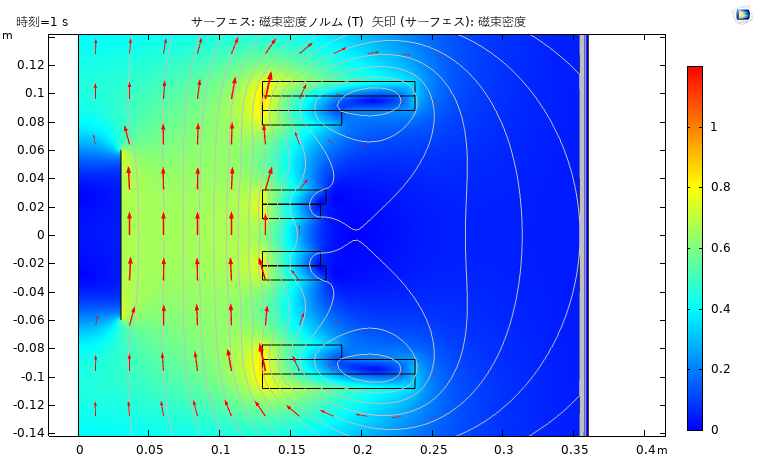
\includegraphics[width=17cm, bb=9 9 900 530]{./section3Effectiveness/BnormDistributionInMRICoilWithoutFM.png}
  \caption{Simulated magnetic field without ferromagnet.}
  \label{fig:simulation_withoutFM}
\end{figure}
\begin{figure}[H]
  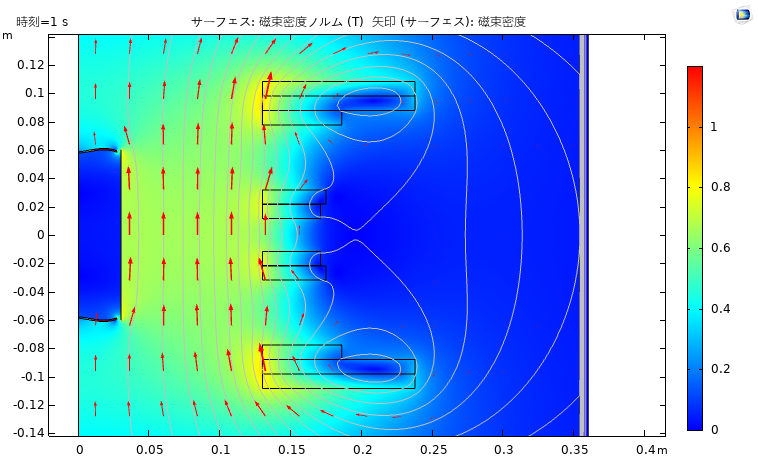
\includegraphics[width=17cm, bb=9 9 900 500]{./section3Effectiveness/BnormDistributionInMRICoilWithFM.png}
  \caption{Simulated magnetic field with ferromagnet.}
  \label{fig:simulation_withFM}
\end{figure}
Comparing the two results,
we can see that the model with ferromagnet actually has reinceforced the outer field near the coil,
and slightly increased the shielding effect on the inner side.
This calculation have confirmed that the inserting ferromagnets on the edge is effective to improve the cloaking ability.

To double check the effect,
an experiment measured the shielding rate along the z axis has been conducted.
The result of measured $B$ field is shown in Fig. \ref{fig:expFMMeasuredBs},
and that of measured shielding rates is shown in Fig. \ref{fig:expFMMeasuredShieldingRates}.
\begin{figure}[H]
  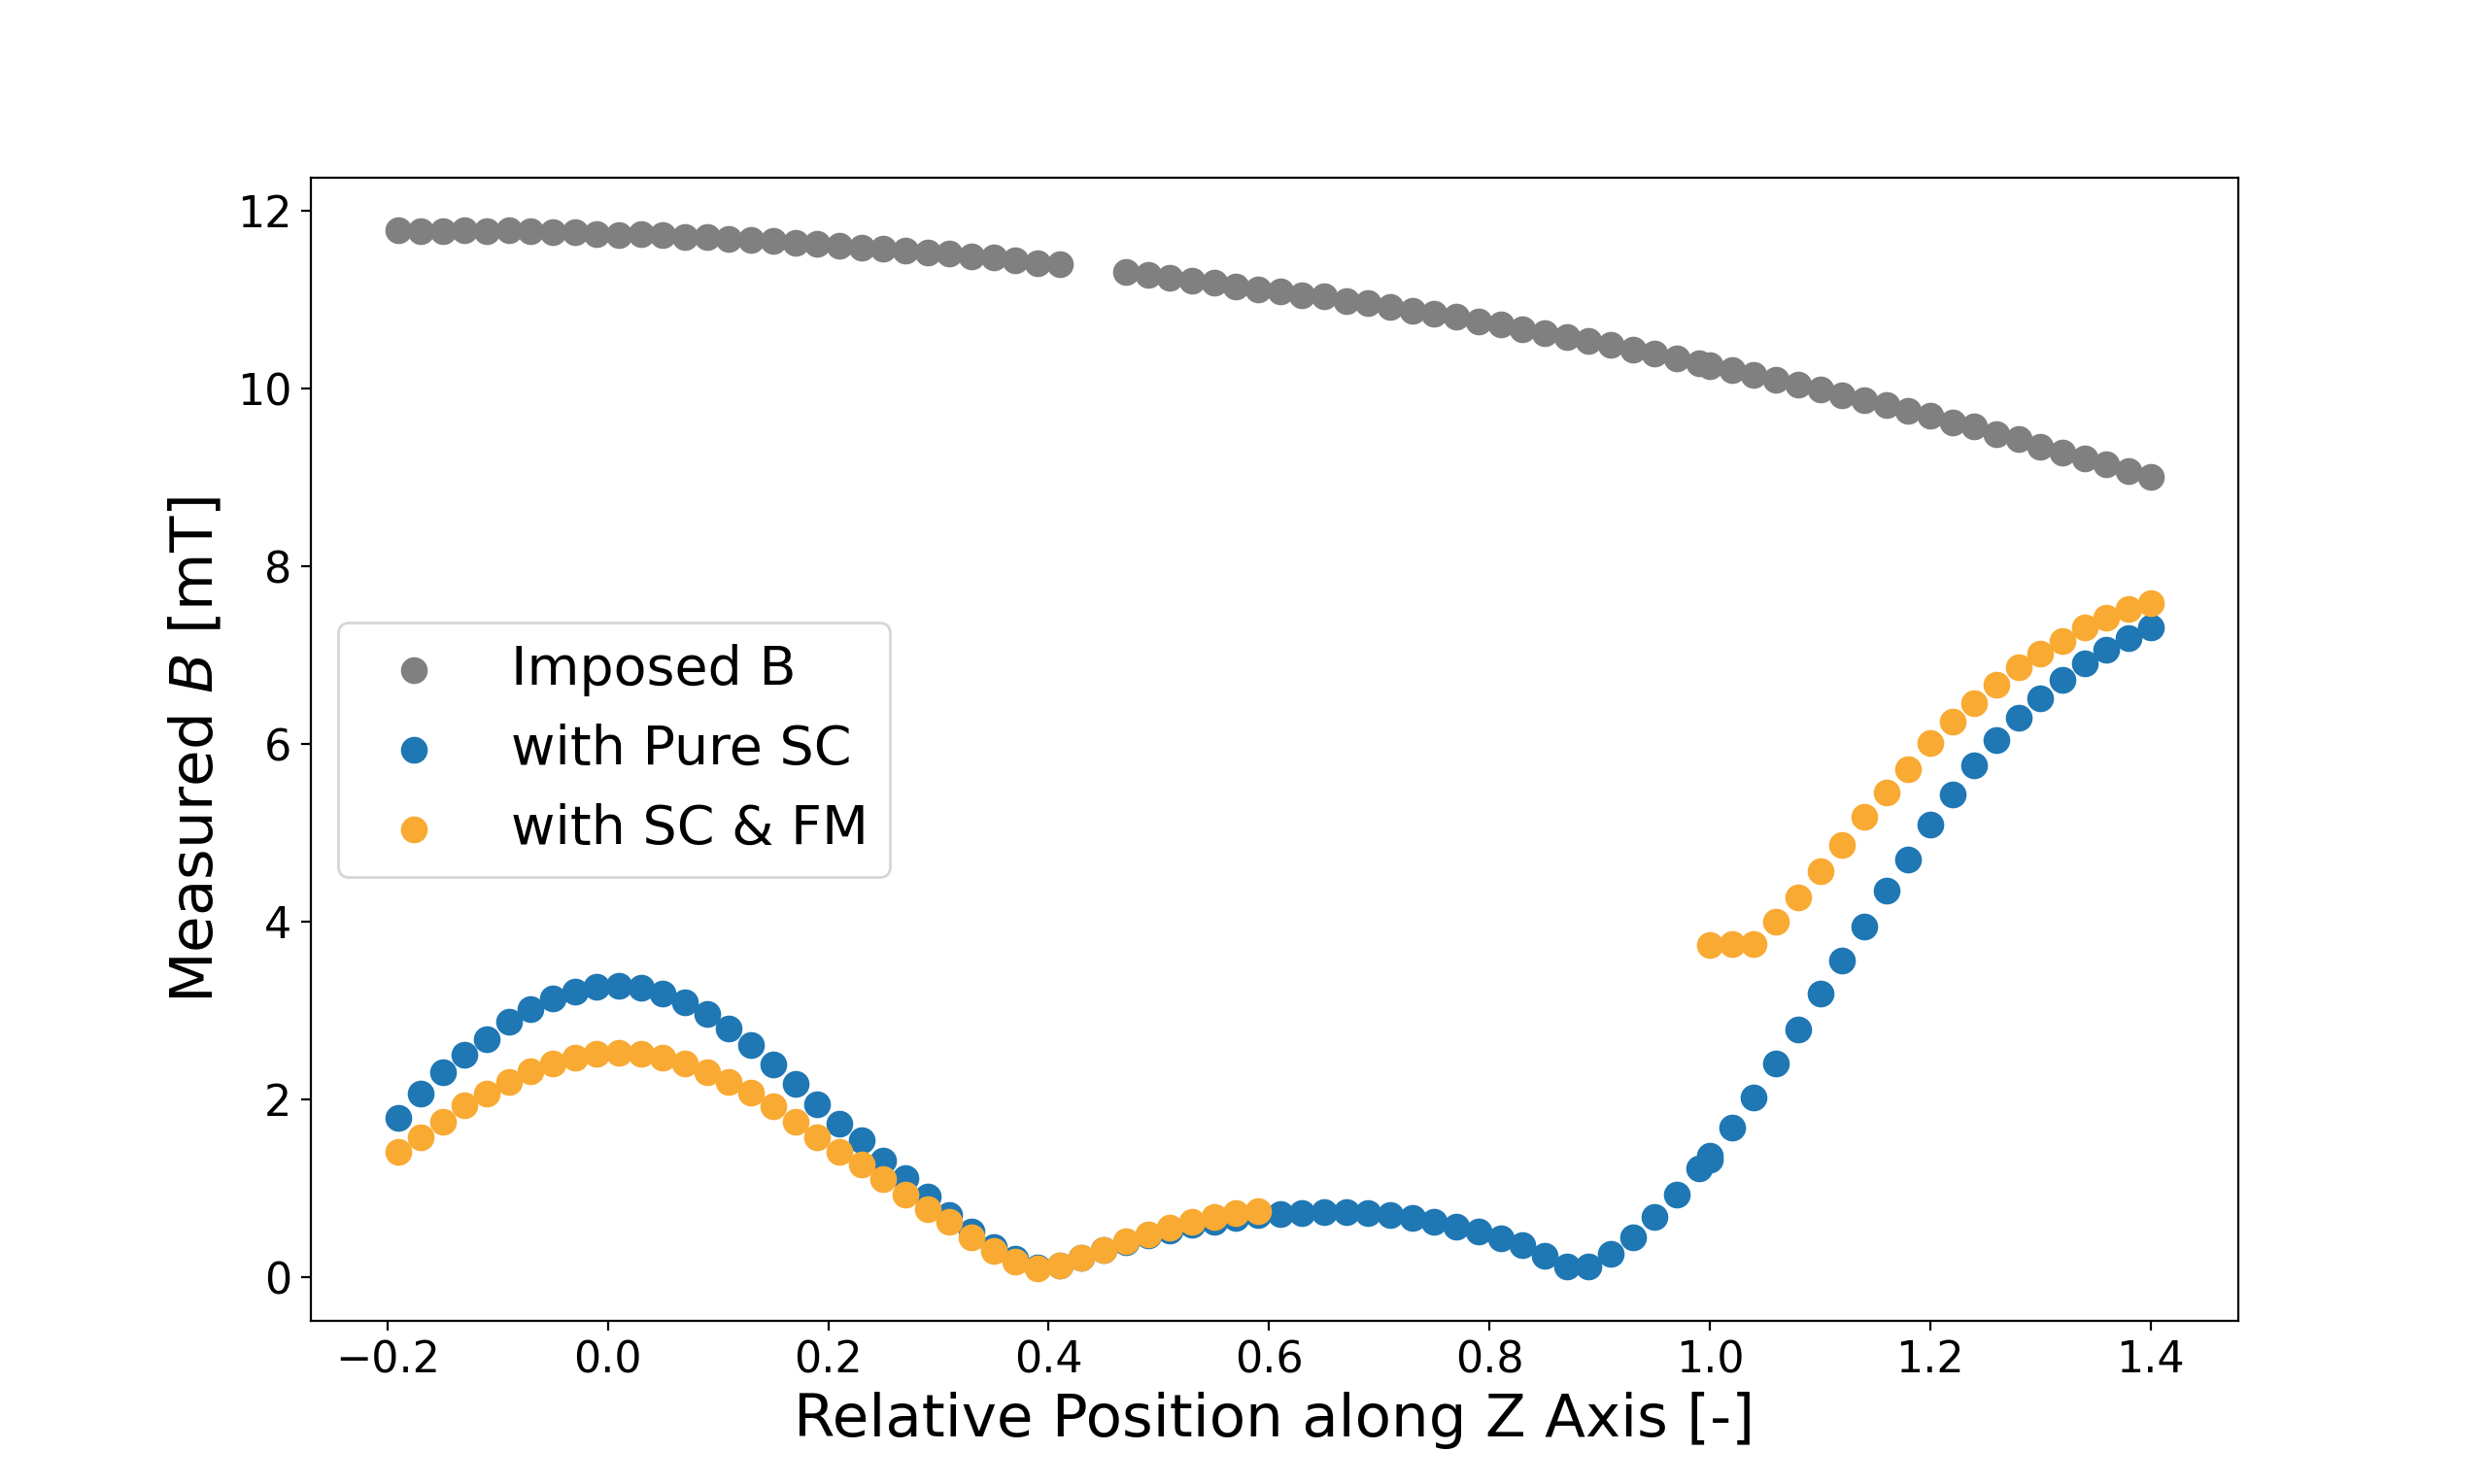
\includegraphics[width=18cm, bb=9 9 900 550]{./section3Effectiveness/comparedB.png}
  \caption{Measured $B$ field along the axis.}
  \label{fig:expFMMeasuredBs}
\end{figure}
\begin{figure}[H]
  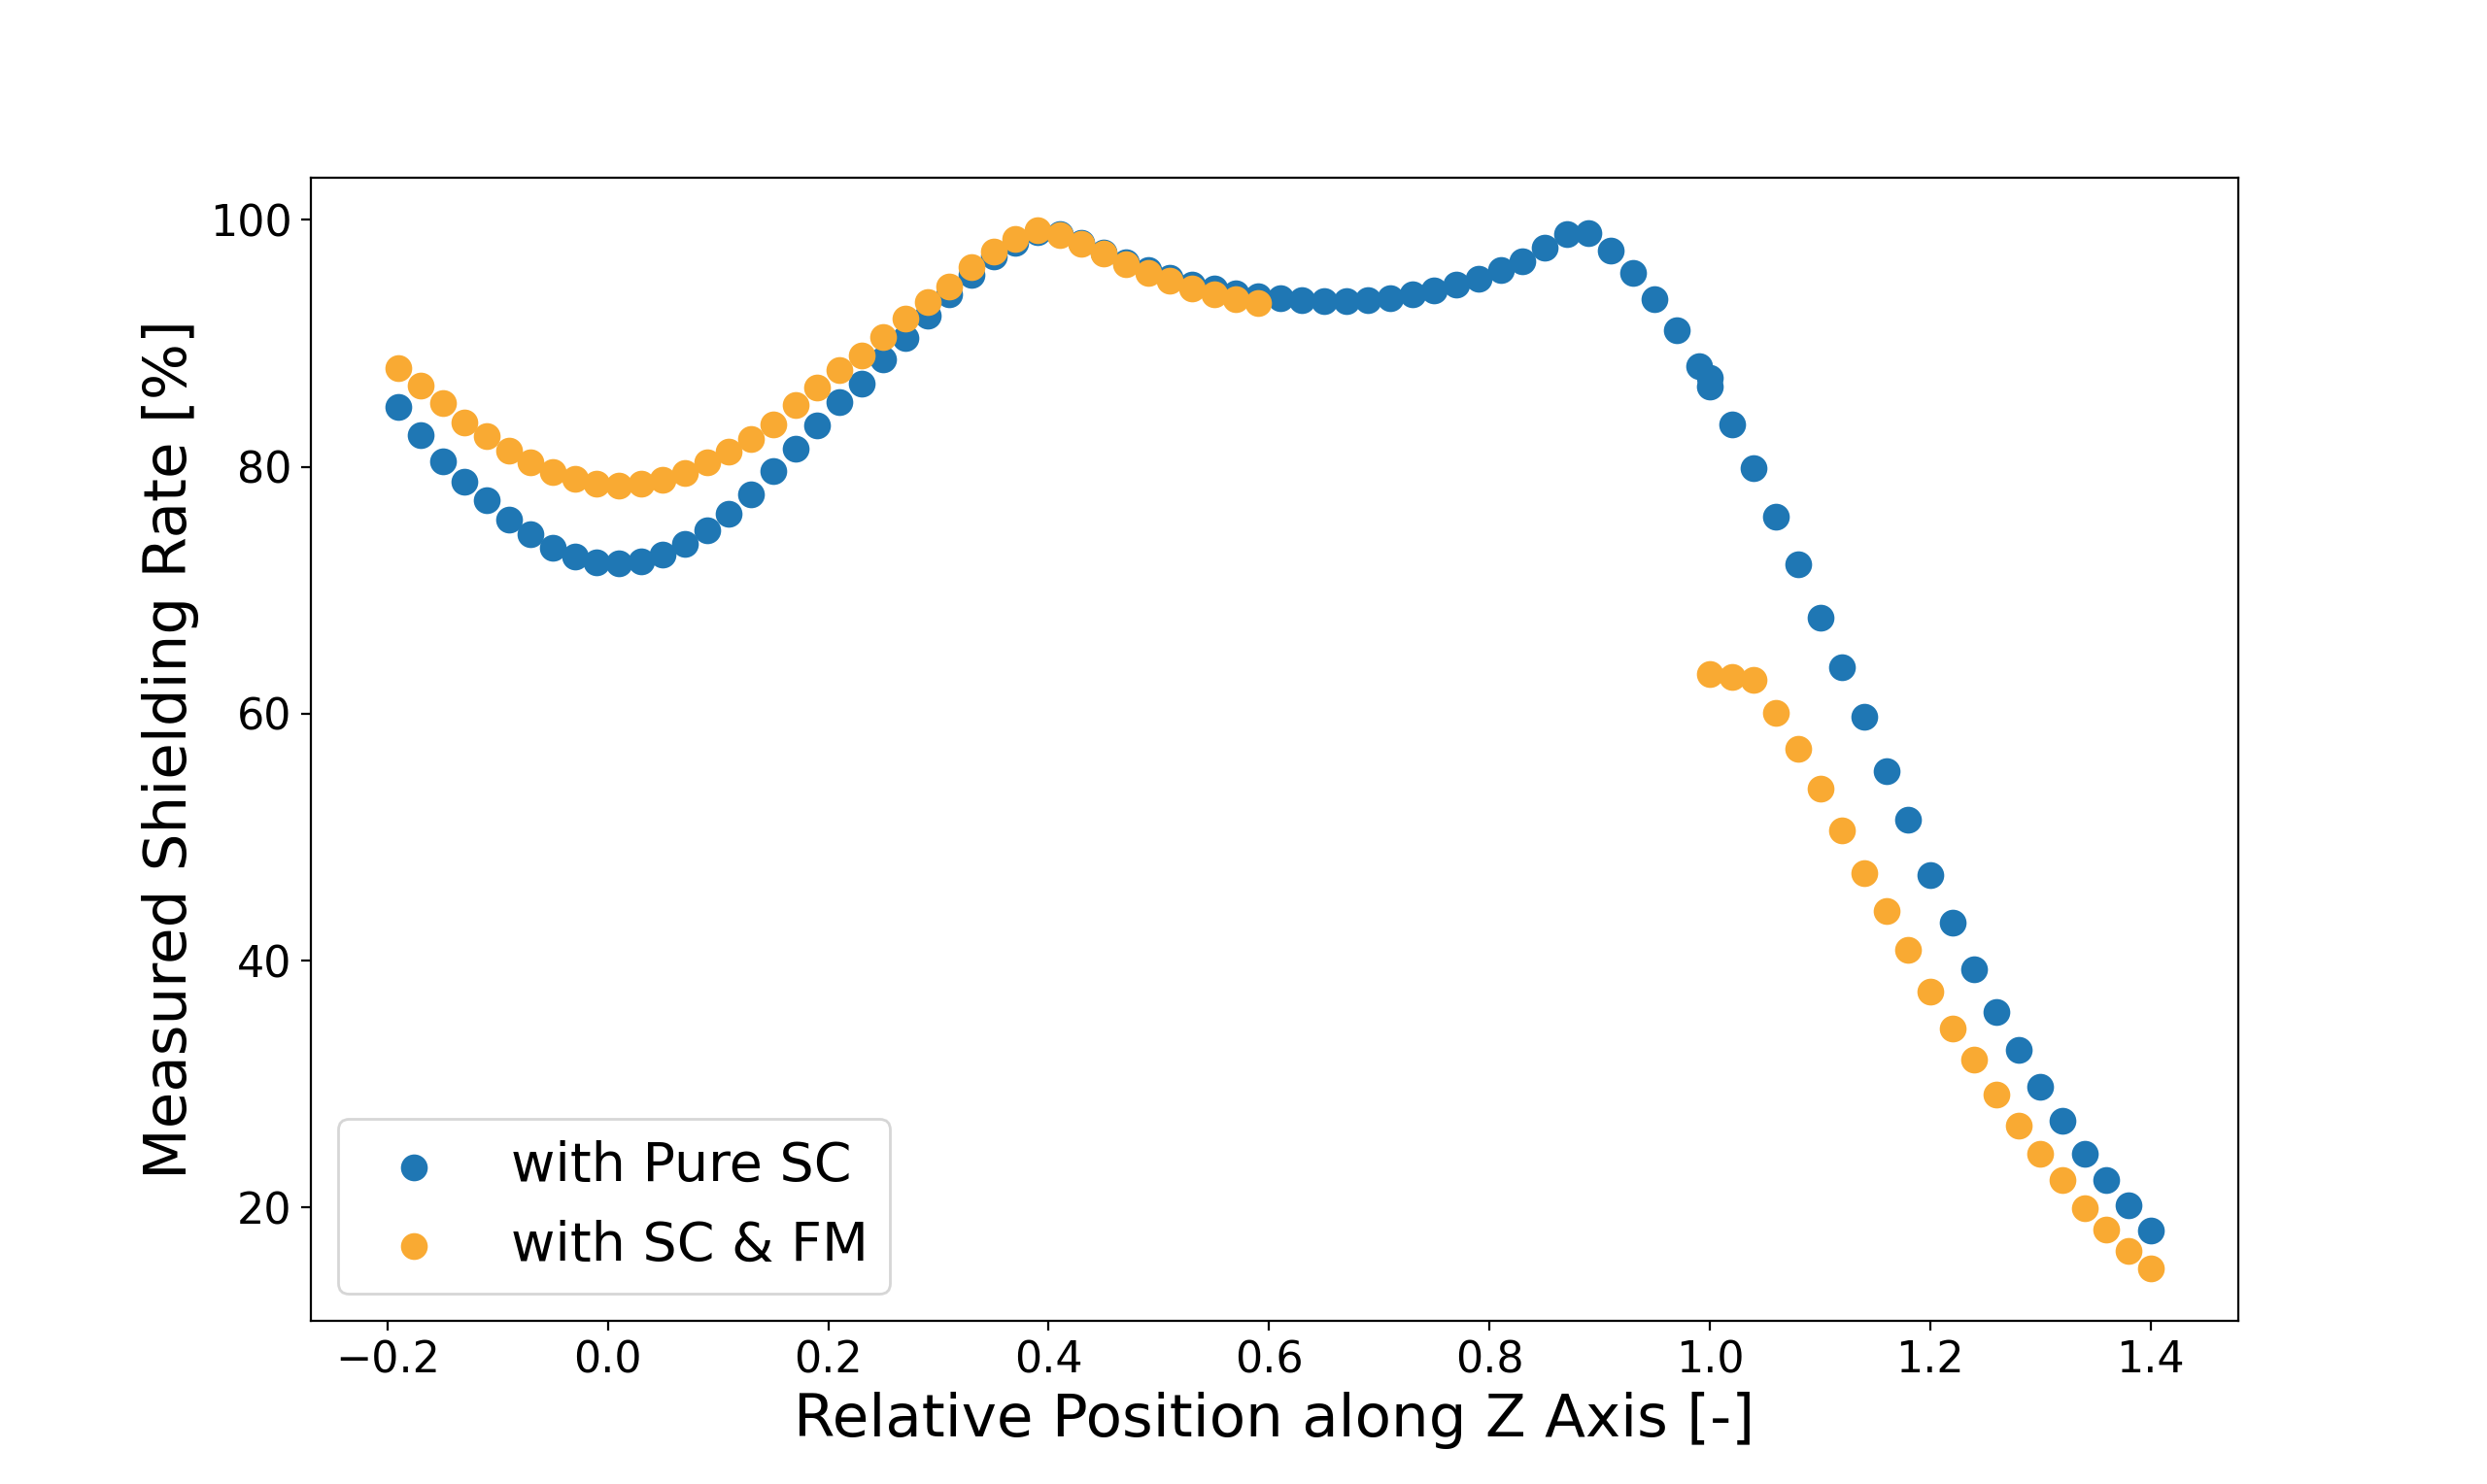
\includegraphics[width=18cm, bb=9 9 900 550]{./section3Effectiveness/comparedShieldingRate.png}
  \caption{Measured shielding rate along the axis.}
  \label{fig:expFMMeasuredShieldingRates}
\end{figure}
From the two figures,
we can seen that with the ferromagnet, the outer field is compensated, and the inner field is further shielded.
This result agrees with the simulated one,
both indicating that placing ferromagnets on the surface of the coil is effective to increase the cloaking ability.


\subsubsection{Conclusion}
In this section, the result of simulation and experiments has shown that placing ferromagnet at the top and bottom surface of the internal coil is able to increase the cloaking ability,
which is to reinforces the outer magnetic field and eliminating the inner magnetic field.
This indicates that a magnetic cloak able to operate in several T field is possible through our proposal using high temperature superconductor tapes and ferromagnets.
To step further,
the optimized construction of the Electromagnetic Induction Type Magnetic Cloak is shown in the next chapter.
